Development of a multi-cellular organism typically starts with a one-cell embryo. This one cell, generated as a result of fertilization (i.e. fusing of the male and female gametes), divides to give rise to the multiple cells and cell types that would eventually form the adult organism. A key question is how the correct arrangement of cells achieved. During development, upto three body axes: anterior-posterior (head-tail), dorsal-ventral (back-front) and left-right, are established. By patterning along these established body axes, proper arrangement of cells can be ensured during development \citep{goldstein1997axis}.

Thus, the body axes serve as the system of spatial axes that allow the embryo to specify position of cells. How are then these body axes established? For many organisms, the embryos start out with few initial asymmetries. Instead, external cues -- such as site of sperm (i.e. male gamete) entry, unequal cell division patterns, and gravity -- are utilized to break the symmetry in the embryo and initiate the establishment of body axes \citep{goldstein1997axis}. Mechanical forces coupled together with chemical patterns translate these external cues into an internal asymmetry of the embryo, by reorganizing certain determinants in the embryo \citep{goldstein1997axis,gross2017active}. As the embryo grows, this unequal distribution of determinants spans across the embryo, thus establishing a body axis \citep{meinhardt2015models,meinhardt2008models}.

It has been observed that the orientation of body axes is relatively fixed with respect to the geometric features of the embryo in many organisms (\autoref{fig:compareBodyAxesEmbryoGeometry}). For example, in many nematodes (roundworms; see \autoref{subfig:compareBodyAxesEmbryoGeometry-apAxisCelegans} for an example in \ac{ce}) the \acl{ap} axis is established at the one-cell stage, and forms along the long axis of the ellipsoidal embryo \citep{goldstein1997axis,goldstein1996specification}. In insect embryos such as fruit flies (see \autoref{subfig:compareBodyAxesEmbryoGeometry-apAxisDrosophila} for an example in \textit{Drosophila}), the \ac{ap} axis forms along the long axis of oocyte \citep{goldstein1997axis,dicko2017geometry,quinlan2016cytoplasmic,shulman2000drosophila,gonzalez1994role}. In chick embryos, Von Baer's rule indicates that the \ac{ap} axis typically forms perpendicular to the long axis of the egg \citep{goldstein1997axis,von1828entwicklungsgeschichte}, but this can be entrained by gravity \citep{kochav1971bilateral}. In mouse embryos (see \autoref{subfig:compareBodyAxesEmbryoGeometry-apAxisMouse}), the \ac{ap} axis initially forms along the axis of the cylindrically-shaped implanted embryo, but then is re-aligned to be along its short axis and transverse to its initial location \citep{tam2004embryonic,vianello2019understanding,hiramatsu2013external,matsuo2017mechanical}. 

\begin{figure}[p]

\centering
\begin{subfigure}{\textwidth}
    \centering
    \includegraphics[width=0.9\textwidth]{Introduction/FigureBodyAxesGeometry/celegans.pdf}
    \caption{\acs{ap} axis in \acs{ce} establishes along the long axis of the ellipsoidal embryo, with posterior half determined by site of sperm entry \citep{goldstein1996specification}. S denotes the sperm at fertilization; AB, P1, ABa, ABp, P2, EMS are names of subsequent blastomeres in embryogenesis (see \autoref{subsec:EarlyEmbryoCelegans} and \cite{strome1989generation}). Top: Sperm enters on the right, away from the female pronucleus -- leading to an embryo with anterior on the left and posterior on the right. Bottom: Sperm enters on the left -- leading to an embryo with anterior on the right and posterior on the left. DV indicates dorso-ventral axis. Adapted from \cite{goldstein1997axis}}
    \label{subfig:compareBodyAxesEmbryoGeometry-apAxisCelegans}
\end{subfigure}
\hfill
\begin{subfigure}{\textwidth}
    \centering
    \includegraphics[width=0.9\textwidth]{Introduction/FigureBodyAxesGeometry/drosophila.pdf}
    \caption{\acs{ap} axis in \textit{Drosophila} is established along the long axis during oogenesis, with posterior half determined by location of oocyte within the germline cyst \citep{gonzalez1994role}. Top: in the usual case, the oocyte migrates towards the posterior of the cyst, specifying the posterior follicle cells that help determine the posterior end. Bottom: if this migration does not occur, no \acs{ap} axis is established. Adapted from \cite{gonzalez1994role}}
    \label{subfig:compareBodyAxesEmbryoGeometry-apAxisDrosophila}
\end{subfigure}
\hfill
\begin{subfigure}{\textwidth}
    \centering
    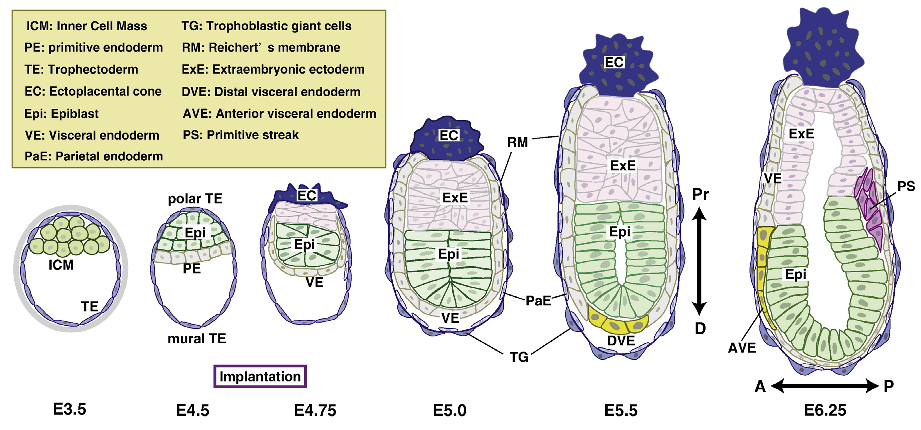
\includegraphics[width=0.9\textwidth]{Introduction/FigureBodyAxesGeometry/mouse.pdf}
    \caption{\acs{ap} axis in mouse is established during uterine implantation. Initial \acs{ap} axis forms along the long axis (Proximal-Distal) of the cylindrical embryo, indicated by the emergence of distal visceral endoderm (DVE) cells at E5.5. \acs{ap} axis reorients to the short axis as the DVE cells migrate to the lateral side, forming anterior visceral endoderm (AVE). Adapted from \cite{matsuo2017mechanical}}
    \label{subfig:compareBodyAxesEmbryoGeometry-apAxisMouse}
\end{subfigure}

\caption[Comparing orientation of \acs{ap} axis with geometry]{Comparing orientation of \acs{ap} axes with embryo geometry in different model organisms: \acs{ce}, \textit{Drosophila}, and mouse}
\label{fig:compareBodyAxesEmbryoGeometry}

\end{figure}

How does this orientation with respect to geometry achieved? Given that mechanical forces are involved in the establishment of body axes, could it be possible that the mechanical forces involved in body axes establishment play a role in achieving this relative orientation? Studies in the mouse embryo seem to suggest so \citep{vianello2019understanding,hiramatsu2013external,matsuo2017mechanical}, but how do mechanical forces enforce this relative orientation is not understood. In this thesis, this problem is studied in the the context of \ac{ap} axis establishment in the \ac{ce} embryo - a nematode. The aim of this thesis is to understand the mechanism(s) that ensure the alignment of the \ac{ap} axis of the \ac{ce} embryo along the long axis of the ellipsoidal embryo. 

In this chapter, the general features of the cytoskeleton in eukaryotic cells are first introduced. The actomyosin cortex, an important higher-order structure of cytoskeletonal elements present in almost all eukaryotic cells, is also described. Next, hydrodynamic theory of active matter is introduced -- the theoretical framework which will be used to model the actomyosin cortex in \autoref{ch:ActiveMatter}. Next, the model organism used in this thesis is introduced: \acl{ce}. The early development of \ac{ce} embryo is described, with focus on the establishment of \ac{ap} axis in the one-cell stage of the \ac{ce} embryo. Next, the phenomenon of \ac{ap} axis alignment -- the active reorientation of the \ac{ap} axis such that it aligns with the geometric long axis of the ellipsoidal embryo -- is described. Possible mechanisms of \ac{ap} axis alignment which have been suggested in previous studies, and explored in this thesis, are described. Finally, an overview of the thesis is provided -- encapsulating the work done in this thesis on elucidating the mechanism of \ac{ap} axis alignment in \ac{ce} embryo.

\section{Cytoskeleton}\label{sec:Cytoskeleton}
As noted above, mechanics plays an important role in the establishment of body axes. Cells thus need to react to the mechanics of their surrounding, and modify their own mechanical properties in response to different stimuli. The structure that allows cells to actively modify their mechanical properties, and perform mechanical tasks, is the cytoskeleton \citep{chaffey2003alberts,bray2001cell,fletcher2010cell}. It is essential in many cellular processes: maintaining cell shape \citep{chaffey2003alberts,rivero1996role,herrmann2007intermediate}, driving locomotion \citep{fletcher2010cell}, and cell division \citep{chaffey2003alberts,gonczy2001spindle}. Its role is to provide the cell with a dynamic mechanical scaffolding, allowing the cell to act as a highly adaptive mechanical entity to achieve different tasks \citep{chaffey2003alberts,bray2001cell,fletcher2010cell}.

The cytoskeleton is commonly defined as a network of protein filaments that extend throughout the cytoplasm of eukaryotic cells, although analogous filaments have also been identified in prokaryotes \citep{erickson2007evolution}. This meshwork of filaments is complemented by motor proteins that exert force betwen the filaments, crosslinking proteins that tie these filaments in the meshwork and various associated proteins that modify and remodel the meshwork \citep{chaffey2003alberts,bray2001cell,fletcher2010cell}. In this section, the elements that make up the cytoskeleton in the eukaryotic cells are introducted. Also introduced is the actomyosin cortex, a thin layer of cytoskeletonal elements present just below the cell membrane \citep{chaffey2003alberts,salbreux2012actin}, and the primary force-generating mechanical structure that this thesis focuses on.

\subsection{Main constituents of the cytoskeleton}\label{subsec:ComponentsCytoskeleton}
\subsubsection{Protein Filaments}\label{subsubsec:FilamentsCytoskeleton}
Protein filaments provide the backbone of the cytoskeleton. In eukaryotic cells, the cytoskeleton is composed of three principal types of protein filaments: actin filaments, intermediate filaments and microtubules. Monomeric protein subunits build each of these filaments. In contrast to usual polymers, these filaments are held together by non-covalent bonds, allowing fast assembly and disassembly \citep{chaffey2003alberts}. 

\paragraph{Actin filaments}
Actin filaments (or F-actin) are right-handed double helix composed of two protofilaments, each being a chain of actin monomers (or G-actin) \citep{pollard1986actin,pollard2000molecular} (see \autoref{subfig:cytoskeletonMainConsituents-actin}). Actin filaments are thin, with a typical diameter of around \SI{7}{\nano\meter} \citep{cooper2007cell}, and flexible, with a typical persistence length of \SI{17}{\micro\meter} \citep{ott1993measurement,gittes1993flexural}. The pitch of the helix formed by the protofilaments is typically around \SI{37}{\nano\meter}. Polymerisation of actin filaments is fueled by hydrolysis of \ac{atp} at the binding site on the monomers as they bind to the filament \citep{fujiwara2007polymerization}. Actin filaments are structurally polar, with a defined (+) or barbed end where new monomers preferentially bind, and a (-) or pointed end where monomers preferentially unbind \citep{pollard1986actin,pollard2000molecular,vavylonis2005actin}. Thus, actin filaments can undergo tread-milling, regulated by \ac{atp} \citep{wegner1982treadmilling}.

Actin filaments often gets organized into higher-order structure, such as the actomyosin cortex (described below), to perform various functions such as migration \citep{pollard2003cellular}, cell division \citep{sanger1975changing} and control of cell shape \citep{clarke1977nonmuscle}. 

\paragraph{Microtubules}
Microtubules are rigid hollow rod-like polymers, formed by the polymerization of a dimer of two globular proteins, $\alpha$-tubulin and $\beta$-tubulin \citep{chaffey2003alberts,nogales1998structure} (see \autoref{subfig:cytoskeletonMainConsituents-microtubule}). These dimers polymerize to form linear protofilaments that associate laterally to form the microtubule \citep{chaffey2003alberts}. Slight offset between protofilaments generates a pseudo-helical structure \citep{hunyadi2007microtubule}. The typical \enquote{\num{13}-\num{3}} arrangement, composed of \num{13} protofilaments with \num{3} dimer offset between neighbouring pairs, has a diameter of approximately \SI{25}{\nano\meter}, and a persistence length of approx \SI{5}{\milli\meter} \citep{chalfie1979organization,chaffey2003alberts,gittes1993flexural,ledbetter1963microtubule} -- practically rigid in most cells, given their typical sizes. Similar to actin filaments, microtubules are also polar, with a fast growing (+) end and a slow growing (-) end \citep{howard2003dynamics}. Microtubules serve various functions such as providing mechanical support, facilitating cell migration and locomotion \citep{mikhailov1998relationship}, acting as pathways for intracellular transport \citep{chaffey2003alberts}, and centering of the mitotic spindle \citep{pearson2004dynamic,grill2003distribution,grill2005theory}.

\textit{Centrosome}: Microtubules usually are nucleated at, and extend outwards from, a \ac{mtoc}, to which the (-) ends are attached. In animal cells, the major \ac{mtoc} is the centrosome, typically present near the nucleus when the cell is not dividing. At mitosis (i.e. when the cell is dividing), the centrosome duplicates \citep{chaffey2003alberts}. In most animal cells, a centrosome consists of a pair of cylinders (centrioles) surrounded by a meshwork of pericentriolar material \citep{pimenta2020pericentriolar}. Complexes of $\gamma$-tubulin in the centrosome serve as the nucleation sites for microtubule assembly \citep{kellogg1994centrosome}. In many animals, centrosomes play an important role in the formation of the mitotic spindle, an array of microtubules and associated proteins responsible for proper segregation of genetic material in the daughter cells after division \citep{bettencourt2013q,chaffey2003alberts}.

\paragraph{Intermediate filaments}
Different cell types also produce other filaments, with a typical diameter of \SI{10}{\nano\meter}. They typically play a structural role and provide mechanical support -- see \cite{chaffey2003alberts,herrmann2007intermediate} for a more detailed review.

\subsubsection{Motor proteins}\label{subsubsec:MotorCytoskeleton}
Motor proteins convert the chemical energy released in \ac{atp} hydrolysis into mechanical work \citep{chaffey2003alberts,bray2001cell,kolomeisky2007molecular,howard2002mechanics}. Motor proteins are categorized into three super-families, distinguished by the type of filaments they bind to. \textit{Myosins} are motors associated with actin filaments, while \textit{kinesins} and \textit{dyenins} bind to microtubules instead \citep{chaffey2003alberts}. Molecular motors perform various functions \citep{chaffey2003alberts}, such as cargo transport \citep{vale2003molecular} and serving as force generators for contraction of large-scale structures \citep{howard2002mechanics,carlsson2006contractile}.

Generally, motor proteins share a common set of \enquote{mechanical parts}: a track on which the motor walks (typically the protein filaments), some fuel (typically \ac{atp}), a transducer and force generator that converts the chemical energy of the fuel into a \enquote{power stroke} to generate mechanical force and a lever that transmits that force to the track \citep{hwang2009mechanical}. This is illustrated using the example of a particular myosin - \acs{nmy2}, which is a major component of the actomyosin cortex. 

\paragraph{\acl{nmy2}}
\ac{nmy2} is a member of the myosin super-family of motor proteins, and therefore a molecular motor that acts on actin filaments (see \autoref{subfig:cytoskeletonMainConsituents-myosin}). It is a major contractile protein of non-muscle eukaryotic cells \citep{chaffey2003alberts,holmes2008myosin}. \ac{nmy2} forms a hexamer consisting of three pairs of polypeptides: two heavy chains, two regulatory light chains involved in regulation of \ac{nmy2} activity and two essential light chains which stabilize the heavy chain conformation \citep{holmes2008myosin,vicente2009non}. Each heavy chain has a motor domain on one end (N-terminus) that binds to actin filament and \ac{atp}, followed by a neck domain to which the regulatory light chains bind, and a coiled-coil domain on the other end (C-terminus) that facilitates dimerization of the heavy chain \citep{holmes2008myosin,vicente2009non,robert2019force}. \ac{nmy2} usually organizes into myosin minifilaments, consists of around \num{28} \ac{nmy2} units \citep{holmes2008myosin,vicente2009non}. 

How does the \ac{nmy2} motor generate force? As depicted in \autoref{subfig:cytoskeletonMainConsituents-powerstroke}, when not bound to \ac{atp} myosin has a strong affinity to actin filament. \ac{atp} binding leads to dissociation of the motor domain from the actin filaments, and \ac{atp} hydrolysis ensues. During this step, the neck domain bends, allowing the motor domain to sample sites on the actin filaments. As myosin binds again to the filament, the products of \ac{atp} hydrolysis are released, resulting in the force generating step (that is, the power stroke) that displaces the motor along the filament with \SI{5}{\nano\meter} displacement, and returns it back to the initial state \citep{de2004relating,sweeney2010structural,tyska2002myosin,robert2019force}. Thus, the motor domains act as the transducer and force generators, the neck domain as the lever, the actin filament as the track and \ac{atp} as fuel for the \ac{nmy2} motor \citep{robert2019force,hwang2009mechanical}. \ac{nmy2} is a non-processive motor (it only makes one step before it detaches from the track \citep{howard2002mechanics,hwang2009mechanical}) with a low duty cycle (fraction of time spent bound to actin filament \citep{howard2002mechanics,hwang2009mechanical}) \citep{kovacs2003functional,wang2003kinetic}. Minifilaments of \ac{nmy2} can slide actin filaments past each other, by creating force dipoles \citep{vicente2009non,niederman1975human,mahajan1996assembly}. \ac{nmy2} also serves as an actin crosslinker \citep{xu2001during,mizuno2007nonequilibrium,laevsky2003cross}.

\begin{figure}[p]

\centering
\begin{subfigure}{\textwidth}
    \centering
    \includegraphics[width=0.9\textwidth]{Introduction/FigureCytoskeleton/actin.pdf}
    \caption{Sketch of an actin filament, red circles denote monomeric G-actin. Arrows indicate rate of chemical reaction at each end. Adapted from \cite{sebastian2012activeChiral}}
    \label{subfig:cytoskeletonMainConsituents-actin}
\end{subfigure}
\hfill
\begin{subfigure}{\textwidth}
    \centering
    \includegraphics[width=0.9\textwidth]{Introduction/FigureCytoskeleton/microtubules.pdf}
    \caption{Sketch of a \enquote{13-3} microtubule, composed of $\alpha$ and $\beta$ tubules. Arrows indicate rate of chemical reaction at each end. Adapted from \cite{sebastian2012activeChiral}}
    \label{subfig:cytoskeletonMainConsituents-microtubule}
\end{subfigure}
\hfill
\begin{subfigure}{\textwidth}
    \centering
    \includegraphics[width=0.9\textwidth]{Introduction/FigureCytoskeleton/myosin.pdf}
    \caption{Schematic of the forms of \acs{nmy2} motor protein. i) \acs{nmy2} converts from inactive state (left) to active state (right) via phosphorylation. Active state has three domains: the globular head containing the motor and actin binding domains, the neck domain or lever arm, and a long coiled-coil domain of heavy chains. ii) \acs{nmy2} can assemble into bipolar filaments -- myosin minifilaments -- and can slide antiparallel actin filaments past each other. Adapted from \cite{vicente2009non}}
    \label{subfig:cytoskeletonMainConsituents-myosin}
\end{subfigure}
\hfill
\begin{subfigure}{\textwidth}
    \centering
    \includegraphics[width=0.85\textwidth]{Introduction/FigureCytoskeleton/powerstroke.pdf}
    \caption{Schematic of the power stroke of \acs{nmy2}. Refer to text for details on power stroke. Adapted from \cite{de2004relating}}
    \label{subfig:cytoskeletonMainConsituents-powerstroke}
\end{subfigure}

\caption[Main constituents of the cytoskeleton]{Main constituents of the cytoskeleton in eukaryotic cells}
\label{fig:cytoskeletonMainConsituents}

\end{figure}

\subsubsection{Associated proteins}\label{subsubsec:AssociatedProteinsCytoskeleton}
Most of the known cytoskeletal proteins are neither filamentenous nor motors. Instead, they modify and interact with the existing protein filaments and motors, to dynamically alter the mechanical properties of the cytoskeleton. A comprehensive overview of the these proteins and their functions is presented in \cite{chaffey2003alberts,pollard1986actin}; here only a brief review of some of the important functions these proteins fulfill is presented.

\textit{Nucleators} help initiate the formation of protein filaments, by providing a nucleation point. \textit{Capping proteins} bind to the ends of filaments, blocking polymerisation at the end where they bind. These proteins thus can either stabilise or de-stabilise a protein filament, depending on where they bind. \textit{Severing proteins} cut filaments. \textit{Crosslinkers} and \textit{bundling proteins} organize protein filaments into structured networks, and modify them. \textit{Sequestering proteins} help with recycling unbound monomers, while \textit{Sidebinding proteins} act as molecular rulers. \textit{Linkers} link filaments of different kinds, allowing different filaments (such as the microtubules and actin filaments) to influence each other. \textit{Regulators} regulate the action of other proteins. Note that individual proteins can have multiple functions, and thus belong to multiple categories.

\subsection{Actomyosin cortex}\label{subsec:ActomyosinCortex}

\begin{figure}[h]
    \centering
    \includegraphics[width=\textwidth]{Introduction/FigureActomyosin/actomyosinSketch.pdf}
    \caption[Sketch of actomyosin cortex]{Sketch of the actomyosin cortex as a quasi-2D polymeric meshwork of actin filaments below the cell membrane (composed of lipids) and interspersed with myosin motors and other proteins. Top represents an effective 2D representation of the actomyosin cortex that could be obtained by averaging over the thickness of the cortex. Adapted from \cite{kumar2021actomyosin}}
    \label{fig:actomyosinCortexSketch}
\end{figure}

The actomyosin cortex, also called the cell cortex, is a thin (around few hundred nanometers \citep{clark2013monitoring}) polymeric meshwork of cross-linked actin filaments, interspersed with myosin motors and associated proteins, that lies just below the cell membrane of most eukaryotic cells \citep{bray1988cortical,chaffey2003alberts} (see \autoref{fig:actomyosinCortexSketch}). Analysis using cryo-electron tomography and atomic force microscopy revealed that actin filaments organize in both isotropic meshworks and actin bundles \citep{hartwig1991cytoskeleton,heuser1980filament,morone2006three,medalia2002macromolecular,pesen2005micromechanical}. 

The cortex is not, however, a static structure -- \ac{atp} hydrolysis fuels the polymerization and de-polymerization of actin filaments, activity of the associated proteins, and force generation by myosin motors. This external energy input and resultant active remodeling of the cortex drives it far from equilibrium, and makes it a very dynamic structure. This highly cross-linked and dynamic nature of the cortex makes it behave like a viscoelastic material \citep{kumar2021actomyosin,salbreux2012actin}, as confirmed by laser ablation experiments \citep{saha2016determining,mayer2010anisotropies}. In live cells, the active remodeling in the cortex occurs on timescales of around \SI{30}{\second} \citep{fritzsche2016actin}, and elastic stresses relax on comparable timescales \citep{saha2016determining}. As a consequence, the cortex can effectively be considered as a viscous fluid on longer timescales. Force generation by myosin motors confer the cortex with a tendency to actively contract \citep{carlsson2006contractile} -- the actomyosin cortex can thus be considered as active viscous fluid.

Actomyosin cortex helps the cell to adapt to changing environmental conditions by controlling cell mechanics. The cortex determines the stiffness of the cell surface, and opposes osmotic pressure \citep{stewart2011hydrostatic}. Global increase in contractility of the cortex facilitates the rounding of the cell before its division \citep{kunda2008moesin}. Local changes in cortex contractility can create gradients of cortical tension. Such changes can aid in cell migration, via retraction of the rear of the cell from the substrate \citep{vicente2009non}. Developmental processes at the tissue scale can also be directed by the cortex of the constituent cells \citep{rauzi2011cortical} -- such as dorsal closure in \textit{Drosophila} \citep{martin2010pulsation} and convergence extension in \textit{Xenopus} \citep{zhou2009actomyosin}. \autoref{sec:ApAxisEstablishment} discusses how local changes in contractility in the one-cell stage \ac{ce} embryo drive flows in the actomyosin cortex of the \ac{ce} embryo, and what role these cortical flows play in the \ac{ap} axis establishment of \ac{ce} \citep{mayer2010anisotropies}.

\section{Hydrodynamic theory of active fluids}\label{sec:introHydrodynamicTheoryActiveFluids}
As discussed in the previous section, the actomyosin cortex can and has been modelled as an active viscous fluid in many previous studies \citep{kumar2021actomyosin,salbreux2012actin,bois2011pattern,saha2016determining,mayer2010anisotropies,fritzsche2016actin,julicher2018hydrodynamic}. General physical principles that govern the behaviour of active biological materials such as the actomyosin cortex can be identified using a hydrodynamic approach \citep{de2013non,julicher2018hydrodynamic,bois2011pattern,gross2017active,reymann2016cortical,kruse2004Asters,salbreux2012actin,julicher2022surface,Kruse2005GenericTO,Prost2015ActiveGP}. By its generic nature, such an approach is not unique to the actomyosin cortex, and has been used to describe other active materials such as bird flocks \citep{toner1995long,toner1998flocks,tu1998sound}, swarms of hydrodynamically interacting swimmers \citep{simha2002hydrodynamic,hatwalne2004rheology}, active polar gels \citep{Prost2015ActiveGP,kruse2004Asters,Kruse2005GenericTO,elgeti2011defect,julicher2018hydrodynamic,julicher2022surface}, active nematic fluids \citep{marenduzzo2007hydrodynamics,fielding2011nonlinear,giomi2011excitable,julicher2018hydrodynamic,julicher2022surface} and active solids \citep{gunther2007spontaneous,banerjee2011instabilities,ranft2010fluidization,julicher2018hydrodynamic}. While the microscopic mechanisms at play in these different active materials can differ considerably, in the hydrodynamic limit -- that is, on large length and long time-scales compared to the microscopic mechanisms of the active material at hand -- general properties of active materials are described by a general hydrodynamic theory corresponding to conservation laws and broken continuous symmetries in the material \citep{julicher2018hydrodynamic,julicher2022surface,Kruse2005GenericTO,Prost2015ActiveGP,de2013non}. In such a theory, a small set of phenomenological coefficients capture the details of the microscopic mechanisms at play in the particular active material under consideration.

This section reviews the general hydrodynamic theory of active fluids based on irreversible thermodynamics. This hydrodynamic theory is a generalization of the hydrodynamics and statistical mechanics of liquid crystals \citep{de1993physics} to systems maintained away from thermodynamic equilibrium by chemical processes driven by fuel(s) provided in external reservoir(s). In the context of the actomyosin cortex, \ac{atp} may serve the role of such a chemical fuel -- utilized by myosin motors to generate mechanical forces in the cortex. Hydrodynamic equations that govern the properties of active fluids can be obtained systematically, by first identifying the conjugate pairs of thermodynamic fluxes and forces. Constitutive material relations can then be expressed via a linear coupling between the thermodynamic fluxes and forces, respecting the Onsager reciprocity relation \citep{onsager1931reciprocalI,onsager1931reciprocalII,mazur1953onsager,casimir1945onsager} and Curie symmetry principle \citep{curie1894symmetry} Phenomenological constants that capture various microscopic processes appear in these constitutive relations. This section closely follows the description presented in \cite{julicher2018hydrodynamic,de2013non,sebastian2012activeChiral}.

At a microscopic level, any active fluid is made up of a large number $N$ of discrete molecules, each with individual mass, position and velocity. A description of the fluid in microscopic details requires that all of the $6N$ degrees of freedoms be tracked, which is infeasible for any active fluid given the large number of molecules involved. Instead, a coarse-grained description of the active fluid is utilized -- in which the fluid is divided into a large number of small volume elements, each of volume $V$. Using this description, densities of molecular components, momentum and energy can be defined for each volume element. To obtain a continuous description of these densities, the continuum limit is considered. Under this limit, the volume $V \rightarrow 0$, with the understanding that the volume still remains large compared to the molecular length scales of the fluid at hand. It is assumed that this continuum limit can always be considered. Altogether, this allows the properties of the active fluid to be described by continuous functions: such as mass density $\rho = \rho(\vec{r})$, flow velocity $\vec{v} = \vec{v}(\vec{r})$ etc. (where $\vec{r}$ is the position vector). The aim of the general hydrodynamic theory reviewed here is to derive dynamic equations for these continuous functions representing the local properties of the active fluid.

Note that Einstein summation is used throughout this section -- summation over repeated indices is implied. Greek alphabet indices assume values $x,y,z$ -- corresponding to the three spatial axes.

\subsection{Conservation Laws}\label{subsec:conservationLaws}
Mass, momentum, angular momentum and energy are conserved quantities, at all scales -- microscopic or macroscopic. This also remains valid in active fluids. Thus, local conservation laws, expressed in terms of the coarsed-grained properties of the active fluid, can be written. 

\subsubsection{Mass conservation}\label{subsubsec:massConserve}
Consider a fixed volume $V$ within the fluid, with boundary $\Omega$, with mass density (mass per unit volume) $\rho$ and flow velocity $\vec{v}$ at any given position $\vec{r}$. Then, the flux of mass flowing out of this fluid is given by:
\begin{equation*}
    \textrm{Mass flux outwards} = \int_{\Omega} \rho \vec{v}\cdot\dd{\vec{\Omega}}
\end{equation*}
However, since mass is conserved within this volume, this flux must match the change in total mass of the volume of fluid. Thus,
\begin{equation*}
    \int_{\Omega} \rho \vec{v}\cdot\dd{\vec{\Omega}} = - \dv{t}\int_V \rho \dd{V} = - \int_V \pdv{\rho}{t} \dd{V}
\end{equation*}
where $t$ is time. The exchange of derivative and integral is allowed since $V$ is fixed. Note that this is true for any arbitrary volume $V$ -- however small or big. Thus, using Gauss' theorem, the following continuity equation can be written:
\begin{equation}\label{eq:introMassBalance}
    \inlinePartial{t}{\rho} + \inlinePartial{\alpha}{\left(\rho v_\alpha\right)} = 0
\end{equation}
The mass flux -- that is, momentum density -- is thus given by $g_\alpha = \rho v_\alpha$

\subsubsection{Energy conservation}\label{subsubsec:energyConserve}
Similar to mass density, an energy density $e$ can be defined for the active fluid. Energy conservation implies that $e$ obeys the following continuity equation:
\begin{equation}\label{eq:introEnergyBalance}
    \inlinePartial{t}{e} + \inlinePartial{\alpha}{\speciesSuper{J}{e}_\alpha} = 0
\end{equation}
where $\speciesSuper{\vec{J}}{e}$ is the energy flux. This flux term can be split into two parts: a convective flux $e\vec{v}$ and a relative flux $\speciesSuper{\vec{j}}{e}$:
\begin{equation}\label{eq:introEnergyFlux}
    \speciesSuper{J}{e}_\alpha = ev_\alpha + \speciesSuper{j}{e}_\alpha
\end{equation}
This relative flux $\speciesSuper{\vec{j}}{e}$ describes the flux of energy in a co-moving reference frame with respect to the volume element at the given position in the fluid. Thus, this relative flux denotes the intrinsic changes in energy density at a given position in the fluid, separate from the changes in energy density caused due to exchange with surrounding volume elements.

\subsubsection{Momentum and Angular Momentum conservation}\label{subsubsec:momentumConserve}
As noted earlier, the momentum density is given by $g_\alpha = \rho v_\alpha$. Momemtum conservation then requires that the following continuity equation is obeyed:
\begin{equation}\label{eq:introMomentumBalance}
    \inlinePartial{t}{g_\alpha} + \inlinePartial{\beta}{\left(g_\alpha v_\beta\right)} = \inlinePartial{\beta}{\sigma_{\alpha\beta}}
\end{equation}
Here, the momentum flux due to convection is $g_\alpha v_\beta$. The total change in momentum of any volume element must match the forces applied onto it on its surface -- which is given by the stress $\sigma_{\alpha\beta}$. Using Gauss' theorem leads to \autoref{eq:introMomentumBalance}.

Similar continuity equations for angular momentum can also be considered -- as presented in \cite{julicher2018hydrodynamic,sebastian2012activeChiral}. However, note that for a non-trivial continuity equation for angular momentum, there must be intrinsic (or spin) angular momentum in the active fluid under consideration. For simplicity, it is assumed that the active fluid under consideration does not have any such intrinsic angular momentum -- both in this section and in \autoref{ch:ActiveMatter}. Thus, angular momentum is conserved, and consequently stress $\sigma_{\alpha\beta}$ is symmetric.

Also, using \autoref{eq:introMassBalance} and \autoref{eq:introMomentumBalance} along with $g_\alpha = \rho v_\alpha$ yields:
\begin{equation}\label{eq:introMomentumBalanceVelocityForm}
    \rho\left(\inlinePartial{t}{v_\alpha} + v_\beta\inlinePartial{\beta}{v_\alpha}\right) = \inlinePartial{\beta}{\sigma_{\alpha\beta}}
\end{equation}

\subsubsection{Particle number conservation}\label{subsubsec:speciesBalance}
The general case of a multi-species active fluid consisting of $N+1$ different species of particles is first considered. In this fluid, the particle number density (number of particles per unit volume) for species $i$ is denoted as $\speciesSuper{n}{i}$, with $i = 0,\ldots,N$. Using the same method as above, the continuity equation for $\speciesSuper{n}{i}$ can be written as:
\begin{equation}\label{eq:introSpeciesBalance}
    \inlinePartial{t}{\speciesSuper{n}{i}} + \inlinePartial{\alpha}{\speciesSuper{J}{i}_\alpha} = \speciesSuper{r}{i}
\end{equation}
where $\speciesSuper{\vec{J}}{i}$ is the flux of particles of species $i$, and $\speciesSuper{r}{i}$ the reaction rate accounting for all the chemical reactions in which species $i$ participates. Note that the number of particles of species $i$ is not conserved in the presence of chemical reactions (that is, a non-zero $\speciesSuper{r}{i}$).

The flux term $\speciesSuper{\vec{J}}{i}_\alpha$ can be split into a convective flux $\speciesSuper{n}{i}v_\alpha$ and a relative flux $\speciesSuper{\vec{j}}{i}$:
\begin{equation}\label{eq:introRelativeSpeciesFlux}
    \speciesSuper{J}{i}_\alpha = \speciesSuper{n}{i}v_\alpha + \speciesSuper{j}{i}_\alpha
\end{equation}
This relative flux $\speciesSuper{\vec{j}}{i}$ describes the movements of species $i$ relative to the volume element at the given position in the fluid -- and thus relative to the local flow of the fluid. Since the mass density can expressed in terms of $\speciesSuper{n}{i}$ as $\rho = \sum_{i=0}^N \speciesSuper{m}{i} \speciesSuper{n}{i}$ (where $\speciesSuper{m}{i}$ is the mass of each particle of species $i$), mass conservation \autoref{eq:introMassBalance} and particle number conservation \autoref{eq:introSpeciesBalance} dictate that:
\begin{equation*}
    \sum_{i=0}^N \speciesSuper{m}{i} \speciesSuper{j}{i}_\alpha = 0, \quad \textrm{and} \quad \sum_{i=0}^N \speciesSuper{m}{i} \speciesSuper{r}{i} = 0
\end{equation*}
with the latter of the two corresponding to the Laviosier's principle of mass conservation in chemical reactions. Using these, the relative flux and reactive rate for one species can be expressed in terms of those for other species. Choosing $i = 0$ yields $\speciesSuper{j}{0}_\alpha = -\frac{1}{\speciesSuper{m}{0}}\sum_{i=1}^N\speciesSuper{m}{i}\speciesSuper{j}{i}_\alpha$ and $\speciesSuper{r}{0} = -\frac{1}{\speciesSuper{m}{0}}\sum_{i=1}^N\speciesSuper{m}{i}\speciesSuper{r}{i}$. Thus, $\speciesSuper{\vec{j}}{0}$ and $\speciesSuper{r}{0}$ can be eliminated. For $M$ linearly independent chemical reactions, additional $M$ relations between the species -- based on the chemical reactions under considerations -- can also be derived. Thus, for an active fluid with $N+1$ species involved in $M$ reactions, $N - M$ independent conservation laws can be obtained for the species number densities $\speciesSuper{n}{i}$. Note that none of the species $i = 0,\ldots,N$ are part of fuel(s) in the external reservoir. For any such fuel species, the above considerations may not apply due to the reservoir. 

For the rest of this discussion, a simpler version of active fluids is assumed -- a three component fluid with the fluid particles, fuel molecules and their reaction products. Furthermore, it is assumed that the concentrations of the fuel and reaction products in the fluid are kept constant via contact with the external reservoir, thus implying $\speciesSuper{\vec{j}}{i} = 0$. The fluid is then kept out of equilibrium by consumption of the chemical fuel at a fixed reaction rate $r$. In the context of the actomyosin cortex, this scenario represents the simplest description of consumption of \ac{atp} (as fuel) by myosin motors -- with the local reaction rate $r$ of \ac{atp} hydrolysis proportional to the local myosin concentration.

\subsection{Continuously broken symmetries}\label{subsec:introLocalOrder}

\begin{figure}
\centering
\begin{subfigure}{0.25\textwidth}
    \centering
    \includegraphics[width=\textwidth]{Introduction/FigureLocalOrdering/isotropic.pdf}
    \caption{Isotropic ordering.\\$\norm{\vec{p}} = 0;\quad \norm{\vec{n}} = 0$}
    \label{subfig:introTheoryLocalOrdering-isotropic}
\end{subfigure}
\hfill
\begin{subfigure}{0.25\textwidth}
    \centering
    \includegraphics[width=\textwidth]{Introduction/FigureLocalOrdering/polar.pdf}
    \caption{Polar ordering.\\$\norm{\vec{p}} = 1;\quad \norm{\vec{n}} = 1$}
    \label{subfig:introTheoryLocalOrdering-polar}
\end{subfigure}
\hfill
\begin{subfigure}{0.25\textwidth}
    \centering
    \includegraphics[width=\textwidth]{Introduction/FigureLocalOrdering/nematic.pdf}
    \caption{Nematic ordering.\\$\norm{\vec{p}} = 0;\quad \norm{\vec{n}} = 1$}
    \label{subfig:introTheoryLocalOrdering-nematic}
\end{subfigure}
\caption[Continuous broken symmetries in complex fluids]{Continuous broken symmetries in complex fluids. The arrows represent the microscopic orientation $\vec{a}$ of the particles that constitute the fluid. The system is in isotropic state in \autoref{subfig:introTheoryLocalOrdering-isotropic} due to the random orientation of $\vec{a}$, in a polar state in \autoref{subfig:introTheoryLocalOrdering-polar} due to the orientation vectors $\vec{a}$ being aligned and parallel and in a nematic state in \autoref{subfig:introTheoryLocalOrdering-nematic} due to the orientation vectors $\vec{a}$ being aligned but anti-parallel.}
\label{fig:introTheoryLocalOrdering}
\end{figure}

In complex active fluids, the constituent molecules can be anisotropic. Many active fluids in biological systems are complex fluids -- such as the actomyosin cortex, in which the actin filaments are structurally polar (see \autoref{subsec:ComponentsCytoskeleton}). Arrangement or bundling of these actin filaments can further break local symmetry -- creating polar or nematic order throughout the fluid. 

In the context of the hydrodynamic theory discussed here, this effect can be captured by endowing each of the constituent particles of the active fluid with an orientation unit vector $\vec{a}$. Note that these orientation vector are a property of each particle -- and is thus not a coarse-grained variable that can be directly used in the hydrodynamic theory. Instead, coarse-grained variables can be derived by inspecting the local distribution of these orientation vectors in a volume element at the position of interest. If all the moments of the local distribution of $\vec{a}$ (that is, within the volume element) vanish, the fluid is isotropic -- and thus does not possess any local order. This is the case for all simple fluid, and with many active fluids. Consequently, locally ordered fluids have non-vanishing moments. 

If the first moment of the local distribution of $\vec{a}$ is non-zero, the fluid has a polar order. For each volume element, a polarity vector $\vec{p}$ can be then defined as the first moment:
\begin{equation}\label{eq:introPolarityVectorDefine}
    \vec{p}(\vec{r}) = \expval{\vec{a}}_{\textrm{Volume element at }\vec{r}}
\end{equation}
where the average is taken in the volume element at the position $\vec{r}$. Under the continuum limit, the polarity vector is a continuous vector function defined at each position and is the coarse-grained order parameter that characterises the local polar order in the active fluid. At any given position, the polarity vector has magnitude of \num{1} if the underlying orientation vectors in the volume element are perfectly aligned and parallel. The polarity vector is $\vec{0}$ for an isotropic fluid, or if the orientation vectors are aligned but anti-parallel. 

If the second moment of the local distribution of $\vec{a}$ is non-zero, the fluid has a nematic order. For each volume element, a nematic tensor $Q_{\alpha\beta}$ can be then defined as the second moment:
\begin{equation}\label{eq:introNematicTensorDefine}
    Q_{\alpha\beta}(\vec{r}) = \expval{a_\alpha a_\beta - \frac{1}{3} \delta_{\alpha \beta}}_{\textrm{Volume element at }\vec{r}}
\end{equation}
where the average is taken in the volume element at the position $\vec{r}$, and the nematic tensor is written for a fluid in 3-dimensions. Under the continuum limit, the nematic tensor $Q_{\alpha\beta}$ is a continuous function defined at each position and is the coarse-grained order parameter that characterises local nematic order in the active fluid. Note that in \autoref{eq:introNematicTensorDefine}, $\vec{a} \rightarrow -\vec{a}$ does not change the nematic tensor $Q_{\alpha\beta}$ -- indicating that the nematic tensor $Q_{\alpha\beta}$ is a measure of the alignment of orientation vectors, but not if those vectors are parallel. Specifically, this implies that the case of orientation vectors being aligned but anti-parallel has a nematic order, but not a polar order. As before, the nematic tensor is zero for an isotropic fluid. 

From the definition in \autoref{eq:introNematicTensorDefine}, one may note that $Q_{\alpha\beta}$ is symmetric ($Q_{\alpha\beta} = Q_{\beta\alpha}$) and traceless ($Q_{\gamma\gamma} = \expval{a_\gamma a_\gamma - \frac{1}{3} \delta_{\gamma \gamma}} = \expval{1 - \frac{3}{3}} = 0$). In the case of uniaxial nematic ordering where $Q_{\alpha\beta}$ has two equal eigenvalues, $Q_{\alpha\beta}$ may instead be written as:
\begin{equation}\label{eq:introNematicTensorUniaxialDefine}
    Q_{\alpha\beta} = S\left(n_\alpha n_\beta - \frac{1}{3}\delta_{\alpha\beta}\right)
\end{equation}
where the unit vector $\vec{n}$ is the nematic director and scalar $S \in [-\flatfrac{1}{2},1]$ corresponds to the degree of alignment of the orientation vectors along the nematic director $\vec{n}$. The nematic director is an eigenvector of the third non-equal eigenvalue of $Q_{\alpha\beta}$. The nematic order of the active fluid may equivalently be represented using the nematic director field. For the isotropic case, $S = 0$; while for the fully aligned case, $S = 1$.

Higher order moments of the local distribution of $\vec{a}$ are usually ignored. In the discussion that follows and in \autoref{ch:ActiveMatter}, the focus is on the nematic tensor $Q_{\alpha\beta}$ and therefore active nematic fluids. Note that as the actomyosin cortex may be considered as an active nematic 2-dimensional fluid on the cell membrane \citep{kumar2021actomyosin,julicher2022surface} (see \autoref{ch:ActiveMatter}). In 2-dimension, only a uniaxial nematic ordering is possible -- as $Q_{\alpha\beta}$ cannot have more than 1 independent eigenvalue.

\subsection{Irreversible thermodynamics of active fluids}\label{subsec:introIrrevThermoActiveFluids}
\subsubsection{Entropy production}\label{subsubsec:introEntropyProduction}
To be able to apply thermodynamic principles to derive the hydrodynamic theory for active fluids, a key assumption of local equilibrium is made. Specifically, it is assumed that each of the volume elements that comprise the active fluid are individually in thermodynamic equilibrium, but out of equilibrium with their neighbours. In this case, the active fluid is locally at equilibrium, but is globally maintained away from equilibrium. Such a local equilibrium can be considered if the small volume elements equilibriate at short times compared to the slow hydrodynamics time scales at large scales. 

Consider now only a single volume element (with volume $V$) at a position $\vec{r}$. Its \enquote{macroscopic} state -- as the volume element is still large enough to contain a large number of constituent particles of the fluid -- is then defined by the various coarse-grained variables defined before, such as: mass density $\rho$, internal energy $e$ and nematic tensor $Q_{\alpha\beta}$ for the active nematic fluid. Under the local equilibrium, one may then define the free energy $F = fV$ and entropy $S = sV$ of this volume element as a function of these coarse-grained variables. Equivalently, for the active fluid, free energy density (free energy per unit volume) $f$ and entropy density (entropy per unit volume) $s$ can be defined. Due to local equilibrium at each volume element, both $s = -\pdv{f}{T}$ and $f = e - Ts$ are valid -- where $T$ is the temperature of the local volume element. Here, only the isothermal case is considered: thus $T$ is the temperature of the whole fluid. Note that the whole fluid is not at equilibrium, in contrast to the locally equilibriated volume elements. However, the fluid's free energy and entropy are well-defined as a sum of local contributions of the locally equilibriated volume elements, and can be expressed in terms of free energy density $f$ and entropy density $s$ as:
\begin{equation}\label{eq:introFreeEnergyEntropyDensityDefine}
    F = \int f \dd{V}; \quad S = \int s \dd{V}
\end{equation}
where the integration is performed over the whole fluid.
 
Consider now the change in the total entropy of the fluid. The change in entropy may be written as a sum of two terms:
\begin{equation}\label{eq:entropyExtrinsicIntrinsic}
    \dd{S} = \dd_{\textrm{e}}S + \dd_{\textrm{i}}S
\end{equation}
where $\dd_{\textrm{e}}S$ is the entropy supplied to the fluid by its surroundings (and thus extrinsic to the fluid), and $\dd_{\textrm{i}}S$ is the entropy produced inside the fluid (and thus intrinsic to the fluid). The second law of thermodynamics states that the irreversible processes in a non-equilibrium system, such as the active fluid, lead to intrinsic production of entropy, implying:
\begin{equation*}
    \dd_{\textrm{i}}S \geq 0
\end{equation*}
with equality only for an equilibrium system. The entropy supplied however can be positive, negative or zero -- depending on the interaction of the fluid with its surroundings. Defining the flux of entropy as $\speciesSuper{\vec{J}}{S}$, and the entropy production rate per unit volume as $\theta$, \autoref{eq:entropyExtrinsicIntrinsic} can be transformed into a continuity equation for the local entropy density $s$:
\begin{equation}\label{eq:introEntropyBalance}
    \inlinePartial{t}{s} + \inlinePartial{\alpha}{\speciesSuper{J}{S}_\alpha} = \theta
\end{equation}
where $\theta > 0$ to satisfy the second law of thermodynamics. Note that $\dd_e S = -\inlinePartial{\alpha}{\speciesSuper{J}{S}_\alpha}$ -- the entropy supplied to the local volume element is related to the entropy flux entering the local volume element. Such a transformation is only possible because of assumption of local equilibrium -- without this assumption, a local entropy density $s$ and entropy production per unit volume $\theta$ do not make sense.

Using \autoref{eq:introEnergyBalance} and \autoref{eq:introEntropyBalance}, along with $f = e - Ts$, one may then write a continuity equation for the free energy density $f$:
\begin{equation}\label{eq:introFreeEnergyBalance}
    \inlinePartial{t}{f} = \inlinePartial{t}{e} - T\inlinePartial{t}{s} = -\inlinePartial{\alpha}{\speciesSuper{J}{e}_\alpha - T\speciesSuper{J}{s}_\alpha} -T\theta \implies \inlinePartial{t}{f} + \inlinePartial{\alpha}{\speciesSuper{J}{f}_\alpha} = -T\theta 
\end{equation}
where $\speciesSuper{\vec{J}}{f} = \speciesSuper{\vec{J}}{e} - T\speciesSuper{\vec{J}}{s}$ is identified as the flux of free energy. Thus, the rate of change of the free energy of the fluid $F = \int f \dd{V}$ for a fixed volume $\mathcal{V}$ of fluid is given by:
\begin{equation}\label{eq:introTotalFreeEnergyTimeDerivativeEntropyProduction}
    \dv{F}{t} = \int_{\mathcal{V}} (-T\theta) \dd{V} + \int_{\partial \mathcal{V}} \speciesSuper{\vec{J}}{f}\cdot\dd{\vec{\Omega}}
\end{equation}
The surface integral term can be interpreted as the work done on the fluid at its surface.

Another way to obtain the rate of change of the free energy of the fluid would be to specify the free energy density $f$. Given the assumption of local equilibrium for each volume element, the free energy per unit volume of the volume element in a co-moving frame can be written. Let this relative free energy density be denoted as $f_0 = f_0(Q_{\alpha\beta},\inlinePartial{\gamma}{Q_{\alpha\beta}})$, which depends on the local nematic tensor and its gradients for the 
active nematic fluid. Then,
\begin{equation}\label{eq:introTotalFreeEnergyDirect}
    f = \frac{g_\alpha g_\alpha}{2\rho} + f_0(Q_{\alpha\beta},\inlinePartial{\gamma}{Q_{\alpha\beta}}); \quad F = \int_{\mathcal{V}} \dd{V} \left(\frac{g_\alpha g_\alpha}{2\rho} + f_0(Q_{\alpha\beta},\inlinePartial{\gamma}{Q_{\alpha\beta}})\right)
\end{equation}
The rate of change of the free energy can then be obtained directly from \autoref{eq:introTotalFreeEnergyDirect}. Comparing the bulk term of the time derivative of free energy thus obtained to \autoref{eq:introTotalFreeEnergyTimeDerivativeEntropyProduction} then yields the entropy production rate per unit volume $\theta$.

\subsubsection{Linear Response theory}\label{subsubsec:introLinearResponse}
In general, the rate of entropy production can be expressed as a sum of products of generalized thermodynamics forces $F_n$ and their conjugate thermodynamic fluxes $J_n$:
\begin{equation}\label{eq:introEntropyProductionGeneral}
    T\theta = \sum_n J_nF_n
\end{equation}
where index $n$ specifies a thermodynamic variable or a tensor/vector component of a given variable. Summation over such an index are explicitly noted here (and thus do not follow the Einstein convention). Equivalently, $J_n$ and $F_n$ can be identified from the expression of rate of entropy production derived previously, using \autoref{eq:introEntropyProductionGeneral}. Note that at equilibrium, all $J_n$ and $F_n$ vanish -- leading to $\theta = 0$, as expected for a system at equilibrium.

Close to equilibrium, the thermodynamic fluxes $J_n$ can be expressed as linear functions of the thermodynamic forces $F_n$:
\begin{equation}\label{eq:introLinearExpansion}
    J_n = \sum_m L_{nm}F_m
\end{equation}
and thus, 
\begin{equation}
    T\theta = \sum_m L_{nm}F_nF_m
\end{equation}
where $L_{nm}$ are Onsager coefficients that capture the active fluid's material properties. Note that $L_{nm}$ themselves can be scalars, vectors or tensors, as is the case with $J_n$ and $F_n$. \autoref{eq:introLinearExpansion} gives the constitutive equations of the material. The second law of thermodynamics requires that $\theta > 0$ for systems not in equilibrium, for all values of the thermodynamic forces $F_n$. Thus, the matrix $L_{nm}$ must be positive definite for the active fluid. This leads to:
\begin{equation}
    L_{nn} > 0; \quad L_{nn}L_{mm} \geq \frac{1}{4}(L_{nm} + L_{mn})^2
\end{equation}
for the diagonal elements $L_{nn}$ and off-diagonal elements $L_{nm}, L_{mn}$.

\subsubsection{Curie symmetry principle}\label{subsubsec:introCurieSymmetry}
In principle, \autoref{eq:introLinearExpansion} allows for any thermodynamic flux $J_n$ to be expressed as a linear function of all thermodynamic forces $F_n$. However, all the fluxes $J_n$ and $F_n$ do not possess the same tensorial character, not do they possess the same symmetry properties. The expansion of a thermodynamic flux $J_n$ into thermodynamic forces $F_n$ must respect the symmetry properties and tensorial character of the flux $J_n$ -- this is the Curie symmetry principle. This principle restricts the choices of $L_{nm}$. For example, in isotropic systems, the Curie principle can be used to show that fluxes and forces of different tensorial ranks do not couple \citep{de2013non}.

\subsubsection{Onsager reciprocity relations}\label{subsubsec:introOnsager}
Another restriction on $L_{nm}$ arises from the Onsager reciprocity relations. These relations arise as a result of invariance under time reversal of microscopic mechanisms. For these relations, the signature $\epsilon$ of the thermodynamic fluxes $J_n$ and forces $F_n$ under time reversal must first be specified. Note that since entropy production $\theta$ has the signature $\epsilon(\theta) = -1$, the signatures of force $F_n$ is opposite to that of its conjugate flux $J_n$: $\epsilon(F_n) = -\epsilon(J_n)$, as a consequence of \autoref{eq:introEntropyProductionGeneral}. From \autoref{eq:introLinearExpansion}, a coefficient $L_{nm}$ couples a flux $J_n$ to a force $F_m$. Thus, the coefficients $L_{nm}$ can be classified based on the signature of the corresponding thermodynamic fluxes and forces they couple: $L_{nm}$ is a reactive coupling if $\epsilon{J_n} = \epsilon(F_m)$, and dissipative if $\epsilon{J_n} = -\epsilon(F_m)$. Reactive coupling are denoted as $L^r_{nm}$, dissipative coupling as $L^d_{nm}$. Then, Onsager reciprocity relations state that:
\begin{subequations}\label{eq:OnsagerRelations}
    \begin{align}
        L^r_{nm} &= -L^r_{mn}\\
        L^d_{nm} &= L^d_{mn}
    \end{align}
\end{subequations}
Note that, by the definition of reactive and dissipative coupling, coupling between a force and its conjugate flux is always dissipative: $L_{nn} = L^d_{nn}$. Essentially, the Onsager relations allow decomposition of the Onsager coefficient matrix $L_{nm}$ into a symmetric dissipative part $L^d_{nm}$ and an antisymmetric reactive part $L^r_{nm}$.

\subsubsection{Hydrodynamics of an active isotropic fluid}\label{subsubsec:introExampleSimpleIsotropicFluid}
The above concepts may be illustrated with an example of an active isotropic fluid. The free energy density of such a fluid is given by $f = \frac{g_\alpha g_\alpha}{2\rho} + f_0$, where $f_0$ is dependent on the fuel that drives this fluid out of equilibrium. Here, the fluid is considered to be under pressure $p$. Then, \autoref{eq:introTotalFreeEnergyDirect} can be written as:
\begin{equation}\label{eq:introActiveSimpleFluidFreeEnergyTotal}
    F = \int \dd{V} \left[\frac{g_\alpha g_\alpha}{2\rho} + f_0\right] - (\textrm{Work done by pressure})
\end{equation}
Note that $f_0$ is a volume term, since the fuel reaction happens in all volume elements. 

As an example, let the activity in this fluid be driven by hydrolysis of \ac{atp} into ADP and $\textrm{P}_\textrm{i}$:
\begin{equation*}
    \textrm{ATP} \rightarrow \textrm{ADP} + \textrm{P}_\textrm{i}
\end{equation*}
Note that this reaction happens at all locations in the fluid. Let $\mu_{\textrm{ATP}}$, $\mu_{\textrm{ADP}}$, $\mu_{\textrm{P}}$ be the chemical potentials for \ac{atp}, ADP and $\textrm{P}_\textrm{i}$ respectively. The change in free energy density in the co-moving frame $f_0$ then can be written as:
\begin{equation}\label{eq:introSimpleActiveFluidFreeEnergyDensityRelative}
    \delta f_0 = \mu_{\textrm{ATP}}\delta c_{\textrm{ATP}} + \mu_{\textrm{ADP}}\delta c_{\textrm{ADP}} + \mu_{\textrm{P}}\delta c_{\textrm{P}}
\end{equation}
where $c_{\textrm{ATP}}$, $c_{\textrm{ADP}}$, $c_{\textrm{P}}$ are the concentrations of \ac{atp}, ADP and $\textrm{P}_\textrm{i}$ respectively. Matter conservation for the chemical reaction above requires that:
\begin{equation}
    \delta c_{\textrm{ATP}} + \delta c_{\textrm{ADP}} = 0; \quad \delta c_{\textrm{ATP}} + \delta c_{\textrm{P}} = 0
\end{equation}
Thus, the rate of change in $f_0$ may be written as:
\begin{equation}\label{eq:introSimpleActiveFluidFreeEnergyDensityRelativeRate}
    \delta f_0 = (\mu_{\textrm{ATP}} - \mu_{\textrm{ADP}} - \mu_{\textrm{P}})\delta c_{\textrm{ATP}} = \Delta\mu\delta c_{\textrm{ATP}} \implies \dv{f_0}{t} = \Delta\mu\dv{c_{\textrm{ATP}}}{t} = - r\Delta\mu
\end{equation}
where $\Delta\mu$ is the difference in chemical potential for the \ac{atp} hydrolysis reaction, and $r = -\dv{c_{\textrm{ATP}}}{t}$ is the rate of consumption of \ac{atp} and thus the reaction rate of \ac{atp} hydrolysis.

Returning to \autoref{eq:introActiveSimpleFluidFreeEnergyTotal}, the rate of work done by pressure (opposing change in volume of each volume element) is given by $p\inlinePartial{\alpha}{v_\alpha} \dd{V}$. From this and \autoref{eq:introSimpleActiveFluidFreeEnergyDensityRelativeRate}, the rate of change of free energy of the fluid can be derived:
\begin{align*}
    \dv{F}{t} &= \int \dd{V} \left[\pdv{t}\left(\frac{g_\alpha g_\alpha}{2\rho}\right) - r\Delta\mu - p\inlinePartial{\alpha}{v_\alpha}\right] = \int \dd{V} \left[\frac{g_\alpha}{\rho}\inlinePartial{t}{g_\alpha} - \frac{g_\alpha g_\alpha}{2\rho^2}\inlinePartial{t}{\rho} - r\Delta\mu - p\inlinePartial{\alpha}{v_\alpha}\right]\\
    &= \int \dd{V} \left[v_\alpha\left(\inlinePartial{\beta}{\sigma_{\alpha\beta}} - \inlinePartial{\beta}{(g_\alpha v_\beta)}\right) + \frac{v_\alpha v_\alpha}{2}\inlinePartial{\beta}{g_\beta} - p\inlinePartial{\alpha}{v_\alpha}  - r\Delta\mu\right]\\
    &= \int \dd{V} \left[v_\alpha\inlinePartial{\beta}{\sigma_{\alpha\beta}} - \left(v_\alpha\inlinePartial{\beta}{(g_\alpha v_\beta)} - \frac{v_\alpha v_\alpha}{2}\inlinePartial{\beta}{g_\beta}\right) - p\inlinePartial{\alpha}{v_\alpha}  - r\Delta\mu\right]
\end{align*}
where \autoref{eq:introMassBalance} and \autoref{eq:introMomentumBalance} have been used, and $g_\alpha = \rho v_\alpha$. Now,
\begin{align*}
    &\frac{v_\alpha v_\alpha}{2}\inlinePartial{\beta}{g_\beta} = \frac{1}{2}\inlinePartial{\beta}{(\rho v_\alpha v_\alpha v_\beta)} - \rho v_\beta v_\alpha \inlinePartial{\beta}{v_\alpha}\\
    &v_\alpha\inlinePartial{\beta}{(g_\alpha v_\beta)} = \inlinePartial{\beta}{(\rho v_\alpha v_\alpha v_\beta)} - \rho v_\alpha v_\beta \inlinePartial{\beta}{v_\alpha}\\
    &\implies v_\alpha\inlinePartial{\beta}{(g_\alpha v_\beta)} - \frac{v_\alpha v_\alpha}{2}\inlinePartial{\beta}{g_\beta} = \frac{1}{2}\inlinePartial{\beta}{(\rho v_\alpha v_\alpha v_\beta)}\\
    &v_\alpha\inlinePartial{\beta}{\sigma_{\alpha\beta}} = \inlinePartial{\beta}{v_\alpha\sigma_{\alpha\beta}} - \sigma_{\alpha\beta}\inlinePartial{\beta}{v_\alpha}
\end{align*}
Using these, the rate of change of free energy is given by:
\begin{equation}\label{eq:introActiveSimpleFluidFreeEnergyRate}
    \dv{F}{t} = \int -\left[\sigma_{\alpha\beta}\inlinePartial{\beta}{v_\alpha} + p\inlinePartial{\alpha}{v_\alpha} - r\Delta\mu\right] \dd{V} + \int \dd{V} \inlinePartial{\beta}{\left[\frac{\rho v_\alpha v_\alpha v_\beta}{2} + v_\alpha \sigma_{\alpha\beta}\right]}
\end{equation}
Comparing to \autoref{eq:introTotalFreeEnergyTimeDerivativeEntropyProduction}, the entropy production rate can be written as:
\begin{equation}\label{eq:introActiveSimpleFluidEntropyProduction}
    T\theta = \sigma_{\alpha\beta}\inlinePartial{\beta}{v_\alpha} + p\inlinePartial{\alpha}{v_\alpha} + r\Delta\mu
\end{equation}

Note that the entropy production is not in the form required by \autoref{eq:introEntropyProductionGeneral} (since at equilibrium neither $\sigma_{\alpha\beta}$ nor $p$ vanish). To do so, the stress tensor $\sigma_{\alpha\beta}$ and velocity gradient $\inlinePartial{\beta}{v_\alpha}$ are decomposed. For $\sigma_{\alpha\beta}$:
\begin{equation*}
    \sigma_{\alpha\beta} = \left[\sigma_{\alpha\beta} - \frac{1}{d}\sigma_{\gamma\gamma}\delta_{\alpha\beta}\right] + \left[\frac{1}{d}\sigma_{\gamma\gamma} + p\right]\delta_{\alpha\beta} - p\delta_{\alpha\beta} = \Tilde{\sigma}^{d,s}_{\alpha\beta} + \sigma^d\delta_{\alpha\beta} -p\delta_{\alpha\beta}
\end{equation*}
where $\Tilde{\sigma}^{d,s}_{\alpha\beta} = \sigma_{\alpha\beta} - \frac{1}{d}\sigma_{\gamma\gamma}\delta_{\alpha\beta}$ is the symmetric traceless part of $\sigma_{\alpha\beta}$, $\sigma^d = \frac{1}{d}\sigma_{\gamma\gamma} + p$ is isotropic part of the stress $\sigma_{\alpha\beta}$ and $d$ is the number of space dimensions. Note that the notation followed here is borrowed from \cite{julicher2018hydrodynamic}. The superscript $d$ refers to the deviatoric part of the stress -- that is, the stress tensor excess from the equilibrium stress. Since for the isotropic fluid, the equilibrium stress tensor is just $-p\delta_{\alpha\beta}$, the above definitions are obtained. For $\inlinePartial{\beta}{v_\alpha}$:
\begin{equation*}
    \inlinePartial{\beta}{v_\alpha} = \left[\frac{\inlinePartial{\beta}{v_\alpha} + \inlinePartial{\alpha}{v_\beta}}{2} - \frac{1}{d}\inlinePartial{\gamma}v_\gamma\delta_{\alpha\beta}\right] + \frac{\inlinePartial{\beta}{v_\alpha} - \inlinePartial{\alpha}{v_\beta}}{2} + \frac{1}{d}\inlinePartial{\gamma}v_\gamma\delta_{\alpha\beta} = \Tilde{v}_{\alpha\beta} + \omega_{\alpha\beta} + \frac{1}{d}\inlinePartial{\gamma}v_\gamma\delta_{\alpha\beta}
\end{equation*}
where $\Tilde{v}_{\alpha\beta} = \frac{\inlinePartial{\beta}{v_\alpha} + \inlinePartial{\alpha}{v_\beta}}{2} - \frac{1}{d}\inlinePartial{\gamma}v_\gamma\delta_{\alpha\beta}$ is the symmetric traceless part of $\inlinePartial{\beta}{v_\alpha}$, $\omega_{\alpha\beta} = \frac{\inlinePartial{\beta}{v_\alpha} - \inlinePartial{\alpha}{v_\beta}}{2}$ is the antisymmetric part of $\inlinePartial{\beta}{v_\alpha}$ and $\frac{1}{d}\inlinePartial{\gamma}v_\gamma$ is the local expansion rate of the fluid. Rewriting \autoref{eq:introActiveSimpleFluidEntropyProduction}:
\begin{equation}\label{eq:introActiveSimpleFluidEntropyProductionOnsager}
    T\theta = \Tilde{\sigma}^{d,s}_{\alpha\beta}\Tilde{v}_{\alpha\beta} + \sigma^d\inlinePartial{\gamma}v_\gamma + r\Delta\mu
\end{equation}
Note that each of $\Tilde{\sigma}^{d,s}$, $\sigma^d$ and $\Delta \mu$ go to zero at equilibrium -- first two because the stress at equilibrium is just $-p\delta_{\alpha\beta}$ and $\Delta \mu$ since at equilibrium the chemical potential difference would be zero (indicating that the hydrolysis reaction does not have preferred direction). Thus, \autoref{eq:introActiveSimpleFluidEntropyProductionOnsager} is in the form of \autoref{eq:introEntropyProductionGeneral}.

Using \autoref{eq:introActiveSimpleFluidEntropyProductionOnsager}, the thermodynamic fluxes and forces can be identified. In here, the choice of forces and fluxes is made are shown in \autoref{tab:introActiveSimpleFluidFluxesForces}. Note that the choice of fluxes and forces is arbitrary -- a force may be treated as a flux and vice versa. Only the pairs themselves are determined by \autoref{eq:introActiveSimpleFluidEntropyProductionOnsager}.
\begin{table}[h]
    \centering
    \begin{tabular}{|c|c|c|c|}
        \hline
        Flux $J_n$ & Force $F_n$ & Time reversal signature $\epsilon(J_n), \epsilon(F_n)$ & Rotation symmetry\\
        \hline
        $\Tilde{\sigma}^{d,s}_{\alpha\beta}$ & $\Tilde{v}_{\alpha\beta}$ & 1,-1 & Traceless symmetric tensor\\
        $\sigma^d$ & $\inlinePartial{\gamma}v_\gamma$ & 1,-1 & Scalar \\
        $r$ & $\Delta \mu$ & -1,1 & Scalar \\
        \hline
    \end{tabular}
    \caption{Conjugate thermodynamic fluxes and forces for a simple isotropic fluid}
    \label{tab:introActiveSimpleFluidFluxesForces}
\end{table}

Using \autoref{eq:introLinearExpansion} and \autoref{eq:OnsagerRelations}, the following can be written:
\begin{subequations}\label{eq:introActiveSimpleFluidOnsager}
    \begin{align}
        \Tilde{\sigma}^{d,s}_{\alpha\beta} &= (L_{11})\Tilde{v}_{\alpha\beta} + (L_{12})\inlinePartial{\gamma}v_\gamma + (L_{13})\Delta \mu\\
        \sigma^d &= (L_{12})\Tilde{v}_{\alpha\beta} + (L_{22})\inlinePartial{\gamma}v_\gamma + (L_{23})\Delta \mu\\
        r &= (-L_{13})\Tilde{v}_{\alpha\beta} + (-L_{23})\inlinePartial{\gamma}v_\gamma + (L_{33})\Delta \mu
    \end{align}
\end{subequations}
where the tensorial character of the Onsager coefficients $L_{11}, L_{12}, L_{13}, L_{22}, L_{23}, L_{33}$ is yet to be determined. Note that since the time reversal signature of $\Tilde{\sigma}^{d,s}_{\alpha\beta}$ and $\inlinePartial{\gamma}v_\gamma$ are opposite, $L_{12} = L_{21}$ is a dissipative coupling, as per Onsager relations. Similarly, since the time reversal signature of $\Tilde{\sigma}^{d,s}_{\alpha\beta}$, $\sigma^d$ and $\Delta\mu$ are the same, $L_{31} = -L_{13}$ and $L_{32} = -L_{23}$ are reactive couplings. Curie principle forces $L_{12} = 0, L_{13} = 0$, as rotation symmetry must match on both sides. Then, $L_{11}, L_{22}$ and $L_{23}$ can be written as scalars, yielding the constitutive equations for an active compressible isotropic fluid:
\begin{subequations}\label{eq:introActiveSimpleFluidConsitutive}
    \begin{align}
        \Tilde{\sigma}^{d,s}_{\alpha\beta} &= 2\eta \Tilde{v}_{\alpha\beta}\\
        \sigma^d &= \eta_v\inlinePartial{\gamma}v_\gamma + \zeta \Delta \mu\\
        r &= -\zeta\inlinePartial{\gamma}v_\gamma + \Lambda \Delta \mu
    \end{align}
\end{subequations}
where the shear viscosity $\eta$ and bulk viscosity $\eta_v$ have been introduced as the Onsager coefficients. $\zeta$ describes the generation of active stress by \ac{atp} hydrolysis, while $\Lambda$ describes diffusion of \ac{atp} and its hydrolysis products. The stress tensor $\sigma_{\alpha\beta}$ can be then written as:
\begin{equation}\label{eq:introActiveSimpleFluidStress}
    \sigma_{\alpha\beta} = \Tilde{\sigma}^{d,s}_{\alpha\beta} + \sigma^d\delta_{\alpha\beta} -p\delta_{\alpha\beta} = \eta \left(\inlinePartial{\beta}{v_\alpha} + \inlinePartial{\alpha}{v_\beta}\right) + \left(\eta_v - \frac{2\eta}{d}\right)\inlinePartial{\gamma}v_{\gamma}\delta_{\alpha\beta} +  (\zeta\Delta\mu - p)\delta_{\alpha\beta}
\end{equation}
\autoref{eq:introActiveSimpleFluidStress} can be used in \autoref{eq:introMomentumBalanceVelocityForm} to obtain the dynamic equation for the flow velocity $\vec{v}$:
\begin{equation}\label{eq:introActiveSimpleFluidMomentumBalance}
    \rho\left(\inlinePartial{t}{v_\alpha} + v_\beta\inlinePartial{\beta}{v_\alpha}\right) = \inlinePartial{\alpha}{(\zeta\Delta\mu - p)} + \eta\inlinePartial{\beta}{\inlinePartial{\beta}{v_\alpha}} + \left(\frac{d-2}{d}\eta + \eta_v\right)\inlinePartial{\alpha}{\inlinePartial{\beta}{v_\beta}}
\end{equation}

Some features of the above derivation may now be recognized. First, note that the coupling between stress and chemical activity in \autoref{eq:introActiveSimpleFluidConsitutive} only exists if the fluid exhibits isotropic stress -- that is, if $\sigma^d$ is not assumed zero throughout. Such a coupling indicates that stresses generated due to fuel consumption lead to expansion or contraction of the volume elements, not shear, in the case of active isotropic fluid. Second, note that the coupling is two-directional -- that is, the reaction rate $r$ is also dependent on the local expansion rate $\inlinePartial{\gamma}{v_\gamma}$ by the same coefficient $\zeta$. As one is typically interested only in the stress tensor $\sigma_{\alpha\beta}$, this effect in the reaction rate is usually not considered. Third, in the specific case of the actomyosin cortex, since the \ac{atp} hydrolysis is catalysed by myosin motors, the active stress $\zeta \Delta\mu$ is typically considered a function of the local myosin concentration on the cortex. 

Finally, consider the case of a bulk 3-dimensional ($d=3$) passive fluid ($r = 0, \Delta \mu = 0$). In this case, \autoref{eq:introActiveSimpleFluidMomentumBalance} reduces to:
\begin{equation}\label{eq:introSimpleFluidNavierStokesCompressible}
    \rho\left(\inlinePartial{t}{v_\alpha} + v_\beta\inlinePartial{\beta}{v_\alpha}\right) = -\inlinePartial{\alpha}{p} + \eta\inlinePartial{\beta}{\inlinePartial{\beta}{v_\alpha}} + \left(\frac{1}{3}\eta + \eta_v\right)\inlinePartial{\alpha}{\inlinePartial{\beta}{v_\beta}}
\end{equation}
For an incompressible fluid passive fluid, $\inlinePartial{\beta}{v_\beta} = 0$ yields:
\begin{equation}\label{eq:introSimpleFluidNavierStokesIncompressible}
    \rho\left(\inlinePartial{t}{v_\alpha} + v_\beta\inlinePartial{\beta}{v_\alpha}\right) = -\inlinePartial{\alpha}{p} + \eta\inlinePartial{\beta}{\inlinePartial{\beta}{v_\alpha}}
\end{equation}
Both of these equations may be recognized as the well-known Navier-Stokes equation of fluid dynamics of a compressible or an incompressible fluid respectively.

\subsection{Constitutive equations of active nematic fluids}\label{subsec:constitutiveEquationsActiveNematicFluids}
Following the principles outlined in this section, constitutive equations for incompressible active nematic fluids have been derived in \cite{julicher2018hydrodynamic}. In particular, the thermodynamic fluxes are identified as (note that the notation followed here is from \cite{julicher2018hydrodynamic}):
\begin{enumerate}
    \item Symmetric traceless part of the deviatoric stress\hfill\\
    Here, deviatoric stress $\sigma^d_{\alpha\beta}$ is defined as the excess stress from the equilibrium (or Ericksen) stress $\sigma^e_{\alpha\beta}$. Such an equilibrium stress arises in nematic fluids due to the free energy $f_0 = f_0(Q_{\alpha\beta},\inlinePartial{\gamma}{Q_{\alpha\beta}})$ for nematic ordering. The symmetric traceless part of this deviatoric stress is written as:
    \begin{equation}\label{eq:introActiveNematicDeviatoricStress}
        \Tilde{\sigma}^{d,s}_{\alpha\beta} = \sigma_{\alpha\beta} - (\sigma^{e,s}_{\alpha\beta} - P\delta_{\alpha\beta}) - (Q_{\alpha\gamma}H_{\beta\gamma} - H_{\alpha\gamma}Q_{\beta\gamma})
    \end{equation}
    where superscript $s$ denotes symmetric part and $\sim$ indicates traceless. $\sigma^{e,s}_{\alpha\beta}$ is the symmetric part of the equilibrium stress, $P$ is the pressure, and $Q_{\alpha\gamma}H_{\beta\gamma} - H_{\alpha\gamma}Q_{\beta\gamma}$ is an antisymmetric stress that arises due to rotational invariance of the free energy in nematic fluids. As indicated before, this antisymmetric component of the stress will be ignored in the theoretical description of the cortex described in \autoref{ch:ActiveMatter}. $H_{\alpha\beta}$ is the molecular field conjugate to the nematic order parameter $Q_{\alpha\beta}$.
    \item Convected co-rotationed time derivative of the nematic tensor\hfill\\
    Convected co-rotationed time derivative is a material derivative taken in a reference frame that is convected and co-rotated with the center of mass of the local volume element \citep{larson1999structure}. It is defined here as:
    \begin{equation}\label{eq:introCorotateDeriveQ}
        \frac{DQ_{\alpha\beta}}{Dt} = \inlinePartial{t}{Q_{\alpha\beta}} + v_\gamma\inlinePartial{\gamma}{Q_{\alpha\beta}} + \omega_{\alpha\gamma}Q_{\gamma\beta} + \omega_{\beta\gamma}Q_{\alpha\gamma}
    \end{equation}
    where $\omega_{\alpha\beta}$ is the vorticity of the fluid, defined as:
    \begin{equation}\label{eq:introVorticityNematic}
        \omega_{\alpha\beta} = \frac{\inlinePartial{\alpha}{v_\beta} - \inlinePartial{\beta}{v_\alpha}}{2}
    \end{equation}
    \item Reaction rate $r$ of \ac{atp} hydrolysis
\end{enumerate}
and the thermodynamic forces are identified as:
\begin{enumerate}
    \item Symmetric traceless part of the Strain rate\hfill\\
    The Symmetric traceless part of the Strain rate $\Tilde{v}_{\alpha\beta}$ is defined as:
    \begin{equation}\label{eq:introActiveNematicStrainRate}
        \Tilde{v}_{\alpha\beta} = \frac{\inlinePartial{\alpha}{v_\beta} + \inlinePartial{\beta}{v_\alpha}}{2} - \frac{1}{d}\inlinePartial{\gamma}{v_\gamma}\delta_{\alpha\beta}
    \end{equation}
    where $d$ is the number of space dimensions of the fluid.
    \item Molecular field conjugate to the nematic tensor\hfill\\
    As noted earlier, $H_{\alpha\beta}$ is the molecular field conjugate to the nematic order parameter $Q_{\alpha\beta}$. It is defined as ($F_0 = \int f_0\dd{V}$):
    \begin{equation}\label{eq:introMolecularFieldDefine}
        H_{\alpha\beta} = -\fdv{F_0}{Q_{\alpha\beta}} = -\pdv{f_0}{Q_{\alpha\beta}} + \inlinePartial{\gamma}{\pdv{f_0}{(\inlinePartial{\gamma}{Q_{\alpha\beta}})}}
    \end{equation}
    \item Chemical potential difference $\Delta\mu$ for \ac{atp} hydrolysis\hfill\\
    Note that the difference between the chemical potential of \ac{atp} and its hydrolysis products remains constant throughout the fluid due to the action of fuel reservoirs, which keep the same concentration of fuel (that is, \ac{atp}) and its products throughout the fluid.
\end{enumerate}
The conjugate pairs of thermodynamic forces and fluxes are listed in \autoref{tab:introNematicFluidFluxesForces}.

\begin{table}[h]
    \centering
    \begin{tabular}{|c|c|c|c|}
        \hline
        Flux $J_n$ & Force $F_n$ & Time reversal signature $\epsilon(J_n), \epsilon(F_n)$ & Rotation symmetry\\
        \hline
        $\Tilde{\sigma}^{d,s}_{\alpha\beta}$ & $\Tilde{v}_{\alpha\beta}$ & 1,-1 & Traceless symmetric tensor\\
        $\frac{DQ_{\alpha\beta}}{Dt}$ & $H_{\alpha\beta}$ & -1,1 & Traceless symmetric tensor \\
        $r$ & $\Delta\mu$ & -1,1 & Scalar \\
        \hline
    \end{tabular}
    \caption{Conjugate thermodynamic fluxes and forces for active nematic fluid. Adapted from \cite{julicher2018hydrodynamic}}
    \label{tab:introNematicFluidFluxesForces}
\end{table}

The constitutive equations for the incompressible active nematic fluid are then written as:
\begin{subequations}\label{eq:constitutiveEqActiveNematic}
    \begin{align}
        \Tilde{\sigma}^{d,s}_{\alpha\beta} &= 2\eta \Tilde{v}_{\alpha\beta} + \nu H_{\alpha\beta} + \zeta Q_{\alpha\beta}\Delta\mu\\
        \frac{DQ_{\alpha\beta}}{Dt} &= -\nu \Tilde{v}_{\alpha\beta} + \frac{1}{\bar{\gamma}} H_{\alpha\beta} + \lambda Q_{\alpha\beta}\Delta\mu\\
        r &= -\zeta Q_{\alpha\beta}\Tilde{v}_{\alpha\beta} + \lambda Q_{\alpha\beta}H_{\alpha\beta} + \Lambda\Delta\mu
    \end{align}
\end{subequations}
Here, $\eta,\nu,\zeta,\bar{\gamma},\lambda,\Lambda$ are phenomenological constants that are material properties of the fluid. Their values are specific to each fluid. Hydrodynamic equations for the fluid can be found by using these equations in the conservation equations such as \autoref{eq:introMomentumBalance}.

In the actomyosin cortex, the \ac{atp} hydrolysis is catalysed by myosin motors to generate mechanical forces (see \autoref{subsec:ComponentsCytoskeleton}). Given the role of myosin as a catalyst for \ac{atp} hydrolysis, the reaction rate $r$ should be dependent on the local concentration of myosin. Such a supposition yields $\zeta$, $\lambda$ and $\Lambda$ as dependent on myosin concentration. Note also that the $\zeta$ and $\lambda$ terms are associated with the nematic tensor, and contribute to deviatoric stress and local change in the nematic tensor respectively. Since the nematic order of the actomyosin cortex is primarily imparted to it by the actin filaments \citep{reymann2016cortical}, $\zeta$ captures the mechanical stress generated by action of myosin motors onto actin filaments and $\lambda$ captures the myosin-driven local alignment of actin filaments. In \autoref{ch:ActiveMatter} this discussion is further expanded on, in the context of \ac{ap} axis alignment.

\section{\acs{ce} as a model organism}\label{sec:CelegansModel}

\begin{figure}[h]
    \centering
    \includegraphics{Introduction/FigureWorm/worm.pdf}
    \caption[\acs{ce} worm and one-cell embryo]{Microscope picture of \acs{ce} worm (top) and one-cell stage embryo (bottom), by M. Leaver (used with permission). A and P mark the anterior and posterior of the developing embryo. Typical location of the one-cell embryo in the gonad of the worm, and its length (approx. \SI{50}{\micro\meter}) is marked}
    \label{fig:celegansWormModelOrganism}
\end{figure}

\acf{ce} was first considered as a potential model organism by Sydney Brenner over \num{50} years ago -- for studies in developmental biology and neuroscience \citep{wb1988nematode,brenner1974genetics,brenner2003nature}.  \ac{ce} is a free-living self-fertilizing transparent nematode, typically found in temperate climate around the world. It is typically a self-fertilizing hermaphrodite with rare spontaneous males (less than \num{0.2}\% of worms \citep{haag2005evolution,corsi2015transparent}) \citep{brenner1974genetics}. It feeds on bacteria, typically \ac{ecoli} on the surface of agarose plates when cultured in lab \citep{brenner1974genetics}. In lab conditions, \ac{ce} worms grow from initial larval stage (\SI{0.25}{\milli\meter} long) to final adult stage (\SI{1}{\milli\meter} long) in around \num{3} days at \SI{20}{\celsius}, although this time can vary with temperature and food available \citep{corsi2015transparent,brenner1974genetics,lee2009regulation}. It is a simple organism in both anatomy and genome. It has a fixed, genetically determined, number of cells at the adult stage, with adult hermaphrodite at 959 somatic cells and adult male at 1033 cells \citep{sulston1983embryonic,kimble1979postembryonic}. One of most prominent features of \ac{ce} is its invariant cell lineage: every worm follows the same pattern of cell divisions and results in the same number of cells, i.e. the developmental fate of every somatic cell is invariant. This has enabled tracing the fate of cell during development, giving rise to a complete map of cell lineage \citep{sulston1983embryonic,sulston1975dopaminergic,kimble1979postembryonic}. Today, there are more than thousand research groups that use \ac{ce} as a model organism, due to the above ease of maintenance and the multitude of biological tools available for study and manipulation of \ac{ce} worms, in various fields such as neuroscience, development, ecology and cell biology \citep{corsi2015transparent}.

Hermaphrodites and males differ in their adult morphology, with males being a bit thinner and shorter, and possess a distinctive tail \citep{corsi2015transparent}. The primary method of reproduction in \ac{ce} is via self-fertilization: hermaphrodites produce both sperms and oocytes, which fertilize each other. A hermaphrodite typically lays about 300 eggs. Males can also fertilize the hermaphrodites, allowing for a form of sexual reproduction. The young worms hatch and subsequently go through four larval stages (L1-L4) before adulthood. These adults are fertile for about \num{3} days, and have an average lifespan of about \numrange{2}{3} weeks \citep{corsi2015transparent}. In harsh conditions, larval development can be paused -- these worms can survive several months in a special state called dauer arrest \citep{hu2007dauer}.

The above properties of \ac{ce} make it very convenient to use as a model organism for development \citep{corsi2015transparent,brenner1974genetics}. It is easy to maintain and grow in bulk due to the large number of progeny and rapid life cycle. Worms can be easily frozen for years and revived later when needed. Individual worms can be easily observed at the level of single cells under the microscope due to their transparency. Its small size allows complete anatomical description even at the electron microscope level. Self-fertilization means a single worm can generate an entire population of its clones, while the rare males, which can be maintained, enable transfer of genetic markers between populations. \ac{ce} is also the first multi-cellular organism with a completely sequenced genome, containing about 18000 predicted genes \citep{c1998genome}. Together with the simple feeding method of double stranded \ac{rnai} in \ac{ce} \citep{kamath2003genome}, all these properties of \ac{ce} make genetic perturbations in \ac{ce} worms a simple and efficient process. Using fluorescent proteins such as \ac{gfp} to tag the proteins in the embryo allows in-depth study of its development \citep{chalfie1994green,boulin2006reporter}.

\subsection{Early embryogenesis in \acs{ce}}\label{subsec:EarlyEmbryoCelegans}

\begin{figure}

\centering
\begin{subfigure}{\textwidth}
    \centering
    \includegraphics[width=\textwidth]{Introduction/FigureEarlyEmbryogenesis/firstCellEvents.pdf}
    \caption{Chronological sequence of events in the one-cell stage embryo, from fertilization until the first cell division. See \autoref{subsec:EarlyEmbryoCelegans} and \autoref{subsec:mechanismApAxisEstablishment} for further details. Anterior is to the left, posterior to the right. Grey circles represent pronuclei and nuclei, black circle extruded polar bodies, purple circle centrosomes. Microtubules are denoted in light grey, arrows illustrate movement. Blue represents \acs{ppar}, red represents \acs{apar}. Adapted from \cite{mirjam2010mechanics}. Also see \cite{schneider2003cell}.}
    \label{subfig:embryogenesisCelegans-onecell}
\end{subfigure}
\hfill
\begin{subfigure}{\textwidth}
    \centering
    \includegraphics[width=\textwidth]{Introduction/FigureEarlyEmbryogenesis/fullEmbryogenesis.pdf}
    \caption{Sketch depicting early embryogenesis in \acs{ce} embryo. The one-cell stage embryo, after fertilization, undergoes an asymmetric division, forming the larger, anterior AB cell and smaller, posterior P1 cell. AB gives rise to somatic cells only. P1 divides further, generating somatic blastomeres EMS (which divides into E and MS), C and D, and the germline progenitor P4. Tissues that the blastomeres give rise to are indicated next to them. Adapted from \cite{mirjam2010mechanics}. Also see \cite{strome1989generation}.}
    \label{subfig:embryogenesisCelegans-full}
\end{subfigure}

\caption[Early embryogenesis in \acs{ce}]{Early embryogenesis in \acs{ce} embryo}
\label{fig:embryogenesisCelegans}

\end{figure}

\ac{ce} embryogenesis begins when a mature oocyte, arrested in meiosis I, is fertilized by a sperm \citep{rose2014polarity,begasse2011} -- see \autoref{subfig:embryogenesisCelegans-onecell}. As discussed more extensively later, the site of sperm entry defines the future posterior end of the embryo \citep{goldstein1996specification} (also, see \autoref{subfig:compareBodyAxesEmbryoGeometry-apAxisCelegans}). Prior to fertilization, the oocyte is fairly symmetric \citep{cuenca2003polarization,cowan2004asymmetric,schonegg2006cdc}. Thus, sperm entry represents the first event in which symmetry is broken in the oocyte. At fertilization, the sperm donates its genetic material -- the male pronucleus -- to the embryo, along with centrosomes \citep{o2000spd,wallenfang2000polarization,cowan2004centrosomes}. After fertilization, meiosis is completed with the extrusion of two polar bodies, usually located at the anterior end. A rigid ovoid-shaped chitin eggshell is secreted by the newly formed embryo after fertilization -- which provides the embryo with its ellipsoidal shape \citep{johnston2012eggshell}.

Events in the one-cell stage of the \ac{ce} embryo -- called the P0 stage -- can be divided into two phases: establishment phase and maintenance phase \citep{cuenca2003polarization}. Establishment phase is initiated by the centrosomes near the male pronucleus. These centrosomes organize microtubule asters, which lead to triggering the establishment of the \ac{ap} axis (discussed later). In the establishment phase, large-scale flows in the actomyosin cortex (directed away from the male pronucleus) and cytoplasm (directed towards the male pronucleus) are observed (which gives the establishment phase its other name -- flow phase). Towards the end of establishment phase, the female pronucleus migrates towards and meets with the male pronucleus, concomitant with a characteristic constriction at the mid of the embryo -- called the pseudocleavage furrow \citep{cuenca2003polarization,nigon1960architecture,reymann2016cortical}. This migration is powered by the microtubules connecting the two pronuclei late in the establishment phase \citep{niwayama2011hydrodynamic}. Pronuclear meeting indicates the end of establishment phase and start of the maintenance phase.

In the maintenance phase, the \ac{ap} axis orientation is maintained -- no flows in the actomyosin cortex or cytoplasm are observed. P granules, which play a role in determining germline fate, localize towards the posterior end, as dictated by the established \ac{ap} axis \citep{gonczy2008mechanisms,hoege2013principles}. The mitotic spindle is set up in the center of the embryo, but elongates towards the posterior end following pronucleus envelope breakdown \citep{grill2003distribution}. The spindle is observed to rock, i.e. oscillate \citep{grill2005theory}. Towards the end of maintenance phase, the P0 cell divides asymmetrically (due to the eccentric location of the mitotic spindle). This results in a large cell towards the anterior and a smaller cell at the posterior, termed AB and P1 respectively. 

These cells divide further as the embryo develops, as depicted in \autoref{subfig:embryogenesisCelegans-full}. The established AP axis is however retained by the distribution of P granules as the embryo develops, as the P granules segregate into the germline precursor cells: P1, P2, P3, P4 \citep{rose2014polarity,strome1989generation}. The P4 cell is the primodial germ cell -- all sperms and oocytes generated in the new worm originate from this P4 cell \citep{rose2014polarity,kimble2005germline}.

\section{\acs{ap} axis establishment in \acs{ce}}\label{sec:ApAxisEstablishment}
In this section, the mechanism of \ac{ap} axis establishment in \ac{ce} is described. As noted before, the \ac{ap} axis is established during the establishment phase at the one-cell stage during \ac{ce} embryogenesis \citep{rose2014polarity}. \ac{ap} axis is established via a cell polarization event mediated by \acs{par} polarity proteins \citep{motegi2013network,hoege2013principles,lang2017proteins}. In this section, the \acs{par} polarity system -- a conserved system of proteins involved in cell polarization in many eukaryotic cells \citep{hoege2013principles} -- is first described. Next, the \ac{ap} axis establishment process is described, detailing the role of the actomyosin cortex and the centrosomal trigger from the male pronucleus. Finally, the phenomenon of \ac{ap} axis alignment is introduced. Mechanisms proposed for \ac{ap} axis alignment by previous studies and considered in this thesis are also described.

\subsection{\acs{par} polarity system}\label{subsec:ParPolarity}
\ac{par} proteins are a conserved set of proteins in eukaryotes, functioning to control asymmetric cell division and partitioning of components in many cell types \citep{goldstein2007proteins,knoblich2001asymmetric}, and crucial in cell polarity establishment \citep{goldstein2007proteins}. \ac{par} proteins were first identified in the \ac{ce} embryos, as a result of genetic mutations that cause symmetric division of the one-cell embryo \citep{guo1995par1,kemphues1988identification}. 

\ac{par} proteins help establish the \ac{ap} axis in \ac{ce} via polarization of the one-cell stage embryo. \ac{par} proteins can be classified into three groups based on their localization in this polarized embryo: PAR-4 and PAR-5 remain uniformly distributed on the cortex, PAR-1, PAR-2, LGL-1 (\ac{ppar}) localize to the posterior half of the cortex and PAR-3, PAR-6, PKC-3 (\ac{apar}) localize to the anterior half of the cortex \citep{motegi2013network}. Importantly, this localization is specific to the cortex (but not absolute) - \ac{par} proteins are uniformly distributed in the cytoplasm \citep{motegi2013network,hoege2013principles}. 

Experiments using Fluorescent Recovery After Photo-bleaching and Fluorescent Correlation Spectroscopy have revealed that \ac{par} proteins can exchange between the cortex and the cytoplasm, and also diffuse laterally on the cortex \citep{hoege2013principles,goehring2011proteins,schubert2000mex,petravsek2008characterization}. Extensive mixing between the \ac{apar} and \ac{ppar} on the cortex is prevented by the mutual inhibition between the two groups: \ac{apar} inhibit the binding of \ac{ppar} to the cortex occupied by \ac{apar}, and vice versa \citep{hoege2013principles,motegi2013network}. The behaviour of \ac{par} proteins on the cortex can be modelled as a reaction-diffusion system, with characteristics similar to those observed \emph{in vivo} \citep{hoege2013principles}. Importantly, \ac{par} proteins can interact with the actomyosin cortex -- \ac{apar} can reduce the dissociation rate of \ac{nmy2} from the cortex \citep{gross2019guiding}, while flows in the cortex can advect the \ac{par} proteins \citep{goehring2011advectionpolarization}. 

\subsection{Mechanism of \acs{ap} axis establishment}\label{subsec:mechanismApAxisEstablishment}

\begin{figure}

\centering
\begin{subfigure}{\textwidth}
    \centering
    \includegraphics[width=\textwidth]{Introduction/FigureApAxisEstablishment/ApAxisEstablishmentEvents.pdf}
    \caption{Schematics depicting the major events that occur in \acs{ap} axis establishment in one-cell \acs{ce} embryo. i) Polarity trigger is provided by the centrosome towards the future posterior end of the embryo, via microtubules and other diffusive components \citep{hoege2013principles}. This trigger displaces the \acs{apar} and down-regulate the actomyosin cortex near the trigger \citep{hoege2013principles,gross2019guiding}. ii) View onto the cell Cortex during \acs{ap} axis establishment. Actomyosin cortex is less cross-linked and less dense in the posterior domain (indicated by \acs{ppar}) compared to anterior domain (indicated by \acs{apar}). The cortex also shows anisotropic tension \citep{mayer2010anisotropies}, with cortical flow directed towards the anterior. Flow speeds are larger in the posterior compared to anterior. iii) Cross-section of the cell cortex. Cortical flows passively transport the \acs{par} proteins by advection \citep{goehring2011advectionpolarization}. Adapted from \cite{hoege2013principles}} 
    \label{subfig:apAxisEstablishmentMechanism-schematics}
\end{subfigure}
\hfill
\begin{subfigure}{\textwidth}
    \centering
    \includegraphics[width=\textwidth]{Introduction/FigureApAxisEstablishment/ApAxisEstablishmentCortexMicrograph.pdf}
    \caption{Cortical activity during \acs{ap} axis establishment. Top: DIC images taken in the midplane of the embryo. Bottom: \acs{nmy2}::\acs{gfp} images taken at the surface of the embryo; that is, in the cortical plane. Anterior is to the left, posterior to the right. $T=$ \SI{0}{\second} indicates start of establishment phase, with myosin forming foci-like structures uniformly in the cortex. After polarization is triggered near the male pronucleus, anterior-directed cortical flows cause the cortex to retrace from the posterior end (ex: $T=$ \SI{225}{\second}). The cortex completely retracts by the time the pseudocleavage furrow forms ($T=$ \SI{495}{\second}), and the two domains have formed. Establishment phase ends at pronuclear meeting ($T=$ \SI{705}{\second}), with myosin foci disappearing from the cortex. Yellow arrows indicate pronuclei (female on the left, male on the right) and blue arrows represent the ingression formed by the pseudocleavage furrow. Scale: \SI{10}{\micro\meter}. Adapted from \cite{sundar2012regulation}}
    \label{subfig:apAxisEstablishmentMechanism-micrograph}
\end{subfigure}

\caption[\acs{ap} axis establishment in \acs{ce}]{Mechanism of \acs{ap} axis establishment in one-cell stage \acs{ce} embryo}
\label{fig:apAxisEstablishmentMechanism}

\end{figure}

\ac{ap} axis establishment starts around \SI{30}{\minute} after fertilization, by the polarity trigger provided by the centrosomes associated with the male pronucleus \citep{o2000spd,wallenfang2000polarization,cowan2004centrosomes,de2020mitochondria}. Before the polarization trigger, the \ac{par} polarity network is primed \citep{zhao2019aurora,reich2019regulated,kapoor2019centrosome,klinkert2019aurora}, resulting in an initially unpolarized one-cell embryo with \ac{apar} uniformly enriched on the cortex \citep{cuenca2003polarization,cowan2004asymmetric,schonegg2006cdc}. 

As the male pronucleus approaches the cortex, the associated centrosome provides the polarity trigger to break this symmetric distribution and initiate \ac{ap} axis establishment \citep{wallenfang2000polarization,hoege2013principles,bienkowska2012centrosomes} -- see \autoref{subfig:apAxisEstablishmentMechanism-schematics}. This polarity trigger loads the \ac{ppar} onto the cortex near the centrosome, and thus near the male pronucleus \citep{wallenfang2000polarization,cowan2004centrosomes,gross2019guiding}. This nascent domain of \ac{ppar}, or the posterior domain, is protected from mutual inhibition from \ac{apar} by microtubules from the centrosome \citep{motegi2011microtubules}. Additionally, the polarity trigger inhibits actomyosin contractility near the male pronucleus by local down-regulation of \ac{nmy2} \citep{motegi2006sequential}. This generates an unequal distribution of myosin motors within the cortex, leading to active stresses in the cortex, and generating flows in the actomyosin cortex towards the future anterior end of the embryo and pointing away from the male pronucleus \citep{munro2004cortical,mayer2010anisotropies}. Cortical flows transport the \ac{par} proteins towards the anterior end via advection -- expanding the posterior domain \citep{goehring2011advectionpolarization}. Difference in the \ac{nmy2} dissociation rates between the posterior and anterior domains \citep{gross2019guiding} further drives the unequal distribution of myosin motors on the cortex, and thus promotes cortical flows. Modification of the actomyosin cortex, and thus cortical flows, can be observed in \ac{nmy2}::\ac{gfp} labelled movies of the \ac{ce} embryo, see \autoref{subfig:apAxisEstablishmentMechanism-micrograph}.

Additional to \ac{par} protein transport, cortical flows also generate cytoplasmic flows due to the drag between the cortex and the cytoplasm; with cytoplasmic flows being directed towards the male pronucleus due to the incompressible nature of the cytoplasm and embryo geometry \citep{niwayama2011hydrodynamic}. Thus, the male pronucleus is pushed into the cortex -- ensuring robust polarization of the embryo \citep{gubieda2020going}. 

Polarization of the embryo thus proceeds via a self-organized mechanochemical feedback loop between the \ac{par} polarity system and cortical flows guided by the polarity trigger from the centrosome \citep{gross2019guiding,bois2011pattern,gross2017active}. \ac{par} proteins control the flows in the cortex \citep{gross2019guiding} and cortical flows control the size of the \ac{par} domains \citep{munro2004cortical,goehring2011advectionpolarization}. Altogether, this process continues until the one-cell embryo is transformed from an initially unpolarized state to a polarized state. The polarization thus set up at the end of establishment phase establishes the \ac{ap} axis -- with the eventual anterior and posterior domains denoting the anterior and posterior end of the embryo. 

Converting this polarization into the \ac{ap} axis is accomplished by processes downstream of the \ac{par} proteins. \ac{par} domains on the cortex induce a cytoplasmic gradient of MEX-5 \citep{schubert2000mex}, which drives the segregation of P granules and various other \enquote{determinants}  towards the posterior end \citep{hoege2013principles}. Differential contractility of the actomyosin cortex in the posterior and anterior domains also sets up the stage for the asymmetric division of the one-cell embryo \citep{grill2003distribution}. Together, these processes ensure that the \ac{ap} axis established at the one-cell stage is realized as the embryo develops.

Note that in the following sections and chapters, unless specifically mentioned, the centrosome is always considered attached to the male pronucleus, and thus the actions of the centrosome are attributed to the male pronucleus as a shorthand.

\subsection{\acs{ap} axis alignment}\label{subsec:ApAxisAlignment}

\begin{figure}

\centering
\begin{subfigure}{\textwidth}
    \centering
    \includegraphics[width=\textwidth]{Introduction/FigureApAxisAlignment/micrograph.pdf}
    \caption{\acs{ap} axis alignment in \acs{ce} embryo, labelled with PAR-2::GFP, PAR-6::mCherry. In the untypical case where the \acs{ap} axis establishment is triggered away from the long axis of the embryo, the \acs{ap} axis -- defined as the orientation of the \acs{par} domains -- reorients towards the long axis of the ellipsoidal embryo. In this micrograph, PAR-2::GFP (in cyan) denotes the posterior domain (\acs{ppar}), and PAR-6::mCherry (in magenta) denotes the anterior domain (\acs{apar}). $T = $ \SI{0}{\minute} denotes the timepoint when the domains are fully established, and the male pronucleus moves away from the cortex. Green dashed circle denotes the male pronucleus. Instantaneous \acs{ap} axis (polarity axis) is denoted by arrow colored cyan to magenta, long axis of embryo is denoted by white arrow. Anterior is to the left, posterior to the right. The timepoints are depicting, in order, the start of establishment phase ($T = $ \SI{-4.0}{\minute}), an intermediate snapshot during cortical flows ($T = $ \SI{-2.5}{\minute}), formation of pseudocleavage furrow ($T = $ \SI{0.0}{\minute}), and pronuclear meeting ($T = $ \SI{3.0}{\minute}). Note the movement of the posterior \acs{par} domain along with the male pronucleus towards the right tip of the embryo -- such that the \acs{ap} axis aligns with the long axis. Images taken by Peter Gross \citep{gross2019guiding} (used with permission)} 
    \label{subfig:apAxisAlignment-micrograph}
\end{subfigure}
\hfill
\begin{subfigure}{\textwidth}
    \centering
    \includegraphics[width=\textwidth]{Introduction/FigureApAxisAlignment/mechanisms.pdf}
    \caption{Possible mechanisms for \acs{ap} axis alignment, driven by cortical flows. Cortical flows can drive flows in the cytoplasm (left) \citep{niwayama2011hydrodynamic} and lead to the formation of a contractile ring of actin around the embryo -- called the pseudocleavage furrow (right) \citep{reymann2016cortical}. Cytoplasmic flow-dependent mechanism (left): In the untypical case where the male pronucleus (green dashed circle) is not on the long axis of the embryo, the polarity trigger (black circle) generates cortical flows (grey arrows) asymmetrically. These leads to asymmetric cytoplasmic flows (black dashed), which can then advect the male pronucleus towards the closest tip (posteriorisation denoted by green block arrow). Pseudocleavage furrow-dependent mechanism (right): In the untypical case where the male pronucleus is not on the long axis of the embryo, the pseudocleavage furrow is generated not perpendicular to the long axis of the embryo. As this contractile ring (black dashed arrows denote contraction) rotates to attain a configuration with minimal length (denoted by grey block arrows), it forces the rotation of the cortex (denoted by grey thin arrows). This forces the male pronucleus towards the closest tip.}
    \label{subfig:apAxisAlignment-mechanisms}
\end{subfigure}

\caption[\acs{ap} axis alignment in \acs{ce}]{\acs{ap} axis aligns to the long axis in one-cell stage \acs{ce} embryo. Possible mechanisms of \acs{ap} axis alignment.}
\label{fig:apAxisAlignment}

\end{figure}

In the description of \ac{ap} axis establishment, the orientation of the \ac{ap} axis with respect to the ellipsoidal-like geometry of the embryo has so far not been considered. The ellipsoidal-like shape is imposed on the embryo by the eggshell surrounding it, which it secretes shortly after fertilization \citep{johnston2012eggshell}. The embryo has one long axis about \SI{50}{\micro\meter} in length, and two short axes about \SI{30}{\micro\meter} in length \citep{begasse2011,riddle1997celegans}. The \ac{ap} axis in \ac{ce} always forms along the long axis of the ellipsoidal embryo \citep{goldstein1996specification}. How then are the \ac{ap} axis and the geometric long axis aligned?

In the typical case, the sperm enters the embryo near long axis of the embryo. Thus, in the typical case, the male pronucleus and the centrosome are located near to the long axis -- ensuring that the \ac{ap} axis already establishes along the long axis. However, as described in \cite{goldstein1996specification}, the \ac{ap} axis will always form along the long axis -- even if the male pronucleus is initially away from the long axis. In this untypical case, which occurs due to lateral sperm entry (sperm entry away from the long axis), the \ac{ap} axis actively re-orient to align with the long axis. As shown in \autoref{subfig:apAxisAlignment-micrograph}, this is observed as the movement of \ac{par} domains to align correctly with the long axis, along with the migration of the male pronucleus with the posterior domain and towards the closest tip \citep{goldstein1996specification}. This migration of the male pronucleus is called here as posteriorisation. The mechanism(s) that drive(s) the alignment of \ac{ap} axis with the long axis is not currently understood.

Multiple mechanisms have been proposed in the past to explain \ac{ap} axis alignment. Observing that the cytoplasmic flows in the embryo are directed towards the male pronucleus, \cite{goldstein1996specification} suggested that these cytoplasmic flows could drive the posteriorization. It was proposed that these flows could push onto the male pronucleus \citep{kimuraCytoplasmicFlows}, and owning to the geometry of the embryo in which the flows operate, push the male pronucleus towards the closest tip in the untypical case \citep{goldstein1996specification} -- see \autoref{subfig:apAxisAlignment-mechanisms}. Experiments with artificially generated cytoplasmic flows in maintenance phase indicate that cytoplasmic flows can influence the orientation of the \ac{ap} axis \citep{mittasch2018non}. Thus, in this mechanism, cytoplasmic flows act as a geometry-sensor. This proposed mechanism of \ac{ap} axis alignment is referred to as the cytoplasmic flow-dependent mechanism. 

In this work, another mechanism for \ac{ap} axis alignment is proposed. In addition to cytoplasmic flows, cortical flows also lead to the formation of the pseudocleavage furrow -- a contractile ring-like structure that forms at the boundary between the two PAR domains late in the establishment phase \citep{nigon1960architecture,reymann2016cortical}. Previous studies have found the pseudocleavage furrow to be not essential for \ac{ap} axis establishment \citep{rose1995pseudocleavage}, but indicate that it may play a role in the dynamics of \ac{ap} axis establishment \citep{aras2018importance}. Here, it is proposed that the pseudocleavage furrow may play a role in \ac{ap} axis alignment. In the untypical case, the pseudocleavage furrow is not perpendicular to the long axis of the embryo. Akin to an elastic rubber-band on an ellipsoid, the pseudocleavage furrow could rotate to minimize its circumference and position itself perpendicular to the long axis, forcing the cortex to reposition such that the \ac{ap} axis aligns with the long axis  -- see \autoref{subfig:apAxisAlignment-mechanisms}. This proposed mechanism of \ac{ap} axis alignment is referred to as the pseudocleavage furrow-dependent mechanism. 

Other mechanisms proposed are concerned with the distribution of \ac{par} proteins, instead of the mechanics-based mechanisms considered above. \cite{gessele2020geometric} proposes that the reaction-diffusion system constituted by the \ac{par} proteins on the ellipsoidal surface of the embryo is sufficient to attain the alignment of \ac{ap} axis with the long axis. However, this mechanism explicitly is considered in the absence of any activity of the actomyosin cortex -- and therefore explains any correction of the \ac{ap} axis during the later maintenance phase, not the alignment in the establishment phase. In fact, previous studies indicate that \ac{ap} axis alignment cannot occur during the establishment phase in the absence of any cortical activity \citep{zonies2010symmetry,motegi2011microtubules,tse2012nop1}. Additionally, \citep{klinkert2019aurora} has indicated that binding and unbinding of \ac{par} proteins to the cortex could be curvature sensitive -- which could also play a role in the geometry sensing required for \ac{ap} axis alignment.

\section{Overview}\label{sec:ApAxisOverview}
The aim of this work is to elucidate the mechanism that drives \ac{ap} axis alignment in the one-cell stage \ac{ce} embryo. This is accomplished in the following way: An active nematic fluid description of the actomyosin cortex present on the 2D surface of the embryo, which can incorporate both the cytoplasmic flow-dependent and pseudocleavage furrow-dependent mechanisms, is first introduced. This theoretical model of \ac{ap} axis alignment, in conjunction with experiments that remove the pseudocleavage furrow, is then used to show that the pseudocleavage furrow-dependent mechanism is the predominant mechanism driving \ac{ap} axis alignment in \ac{ce}, with cytoplasmic flow-dependent mechanism a minor contributor. Furthermore, relation between \ac{ap} axis alignment and embryo geometry is explored. Experimental modifications to the embryo geometry are used to show that embryo geometry can influence \ac{ap} axis alignment process in a manner consistent with both the theoretical description of the cortex and a simplified model of the pseudocleavage furrow-dependent mechanism. 

The structure of the thesis is as follows. In \autoref{ch:ActiveMatter} the theoretical model of \ac{ap} axis alignment is introduced, developed by combining the descriptions of the cortex from \cite{gross2019guiding} and \cite{reymann2016cortical}. Details on the numerical simulations and selection of parameters of the theoretical model are also briefly described. In \autoref{ch:Exp}, the experimental methods of the work presented in this thesis are detailed, alongwith discussing the worm strains used and genetic perturbations made. Details of acquiring movies of \ac{ce} embryos undergoing \ac{ap} axis alignment, and their subsequent analysis to obtain relevant measurements are also discussed. In \autoref{ch:Results}, the tools introduced in \autoref{ch:Exp} are used to test various hypotheses experimentally and compare their results to simulation results from the theoretical model discusses in \autoref{ch:ActiveMatter}, in order to elucidate the mechanism of \ac{ap} axis alignment. In \autoref{ch:Summary}, the results presented in this thesis are summarised and discussed in context of results from previous studies. 

